\documentclass[a4paper]{article}
\usepackage{graphicx}
\graphicspath{{./figures/}}
\usepackage[italian]{babel}
\usepackage{float}
\usepackage{braket}
\usepackage{listings}
\usepackage{minted}
\usepackage{mdframed}
\usepackage{tikz}
\usepackage{enumitem}
\usetikzlibrary{shapes, arrows, automata, petri, decorations.markings, decorations.pathreplacing, positioning, calc}

\usepackage{hyperref}
\hypersetup{
  colorlinks=false,
}

\newcommand{\mycomment}[1]{}

% Code blocks
\definecolor{codegreen}{rgb}{0,0.6,0}
\definecolor{codegray}{rgb}{0.5,0.5,0.5}
\definecolor{codepurple}{rgb}{0.58,0,0.82}
\definecolor{backcolour}{rgb}{0.95,0.95,0.95}

\lstdefinestyle{mystyle}{
  backgroundcolor=\color{backcolour},
  commentstyle=\color{codegreen},
  keywordstyle=\color{magenta},
  numberstyle=\tiny\color{codegray},
  stringstyle=\color{codepurple},
  basicstyle=\ttfamily\footnotesize,
  breakatwhitespace=false,
  breaklines=true,
  captionpos=b,
  keepspaces=true,
  numbers=left,
  numbersep=5pt,
  showspaces=false,
  showstringspaces=false,
  showtabs=false,
  tabsize=2
}

\lstset{style=mystyle}

\begin{document}

% Title ------------------------------------------------------------------------------
\title{Documentazione progetto Ingegneria del Software\\[1ex]
  \large Software di gestione dei pazienti diabetici
}

\author{
  \vspace{0.8cm}
  Università di Verona\\
  Imbriani Paolo - VR500437\\
  Irimie Fabio - VR501504
}

\begin{figure}
  \centering
  
\includegraphics[width=0.3\textwidth]{UniversityofVerona}
\end{figure}

\maketitle 

\pagebreak
% Title ------------------------------------------------------------------------------

\tableofcontents

\pagebreak

\section{Requisiti e Use Case}

\subsection{Note generali}

Il software che si andrà a sviluppare è un sistema di telemedicina di un servizio clinico per la gestione
di pazienti diabetici. Gli attori principali del sistema sono i \textit{medici} (diabetologi) e i \textit{pazienti}; questi ultimi
hanno credenziali di accesso al sistema fornite dagli amministratori del servizio con cui possono autenticarsi.
Se l'autenticazione va a buon fine allora l'utente verrà indirizzato alla propria \textit{home page} in cui potrà
visualizzare le informazioni relative al loro ruolo. Nel seguente diagramma dei casi d'uso sono rappresentati
i principali attori e le loro interazioni con il sistema. Notare che diamo per scontato che tutti gli autori siano già autenticati
per semplificare il diagramma.

\begin{figure}[H]
  \centering
  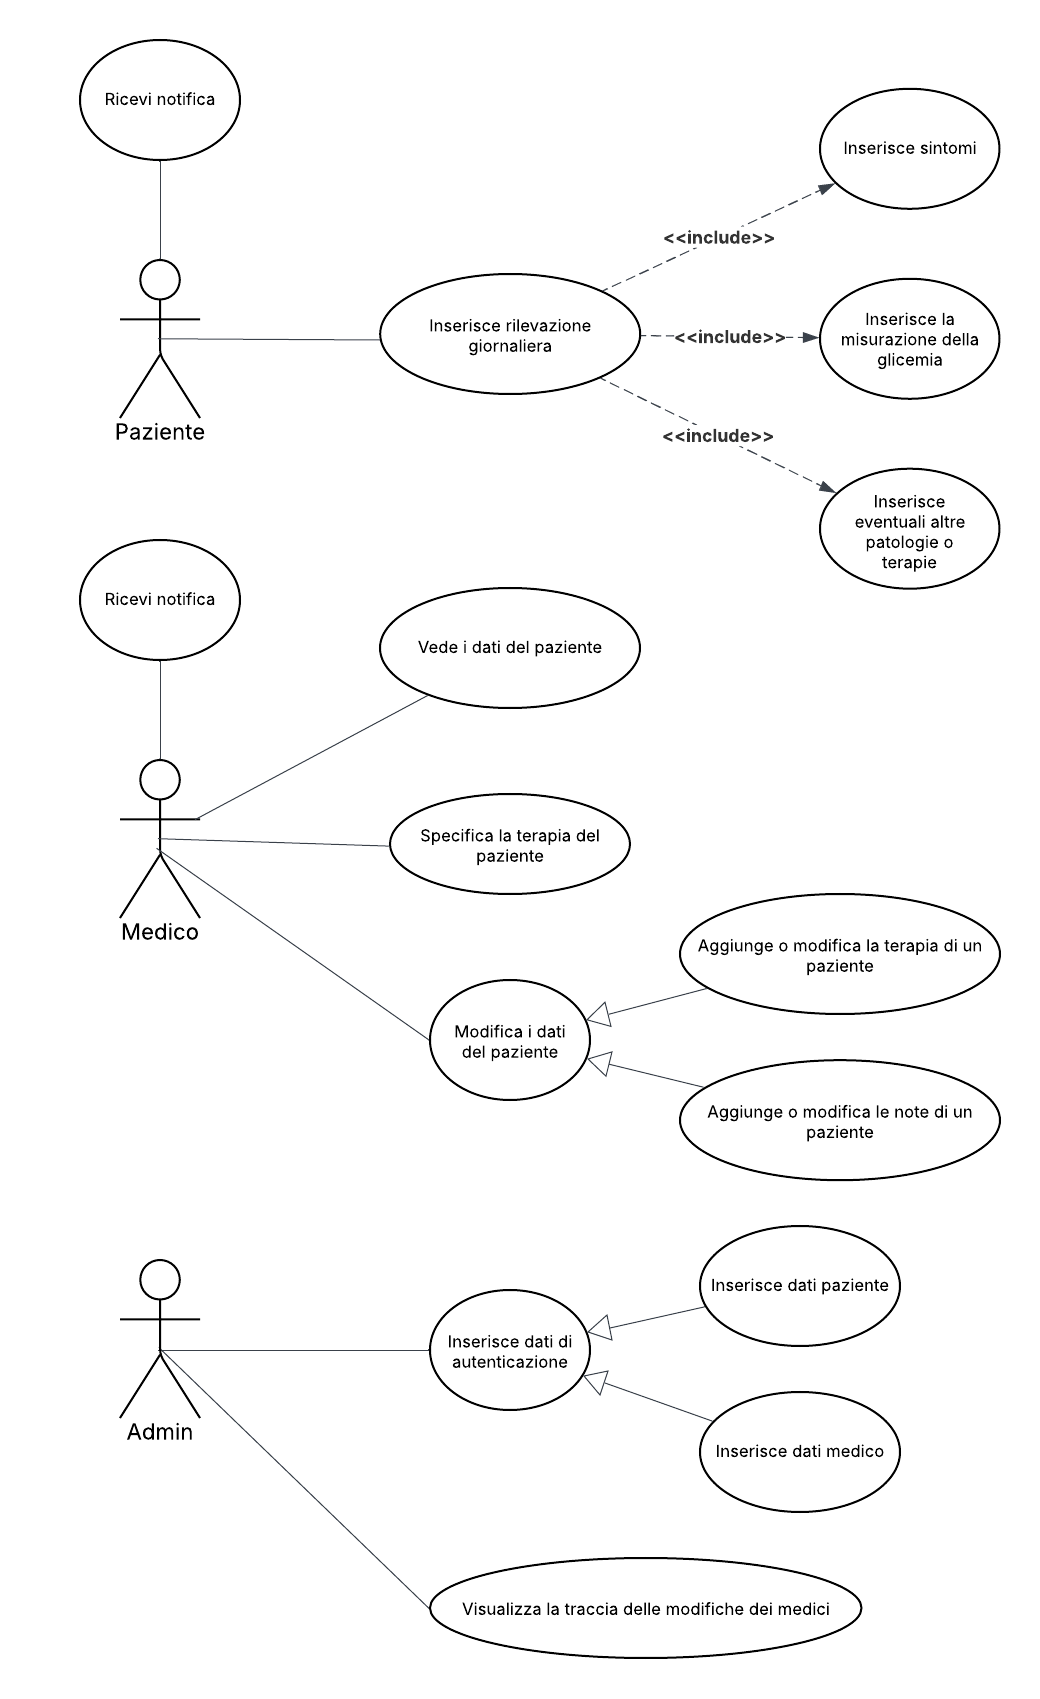
\includegraphics[width=0.7\textwidth]{usecase}
  \caption{Diagramma dei casi d'uso}
  \label{fig:usecase}
\end{figure}

\subsection{Casi d'uso del paziente}

Una volta che il paziente si è autenticato ed è entrato all'interno della sua area riservata, egli può
inserire i dati giornalieri relativi alla sua glicemia (prima e dopo ogni pasto); per fare questo
ha bisogno di inserire dati quali: sintomi, rilevazione glicemica, eventuali altre patologie o terapie.

\subsubsection{Inserimento dei dati giornalieri}

\begin{mdframed}
  \textbf{Attore}: Paziente\\
  \textbf{Precondizioni}: Il paziente deve essere autenticato\\
  \textbf{Passi}: 
  \begin{enumerate}[nosep]
    \item Il paziente accede alla sua home page
    \item Il paziente entra dentro l'area di inserimento dei dati giornalieri
    \item  Il paziente inserisce il dato della sua glicemia prima pasto e dopo pasto
      \begin{itemize}
        \item  Il paziente può aprire un ulteriore finestra per inserire i sintomi, le terapie e le patologie, con oppurtuna data 
        \item  Può anche inserire le assunzioni di insulina o qualsiasi farmaco prescritto dal diabetologo, specificandone giorno, ora, farmaco e quantità assunta
      \end{itemize}
    \item Il paziente inserisce la data e ora di rilevazione
    \item Il paziente conferma l'inserimento dei dati
  \end{enumerate}
  \textbf{Postcondizioni}: La rilevazione è inserita 
\end{mdframed}
\noindent
Andiamo a specificare come viene gestito \textbf{l'inserimento dei dati} del paziente: i dati glicemici sono quelli
che il paziente inserisce giornalmente e obbligatori per inviare le rilevazioni. Dopo aver inserito i dati, l'utente può anche:
\begin{itemize}
  \item inserire specifiche sulla patalogia, terapia o sintomi
  \item inserire le assunzioni di insulina o qualsiasi altro farmo prescritto dal diabetologo
\end{itemize}

\begin{figure}[H]
  \centering
  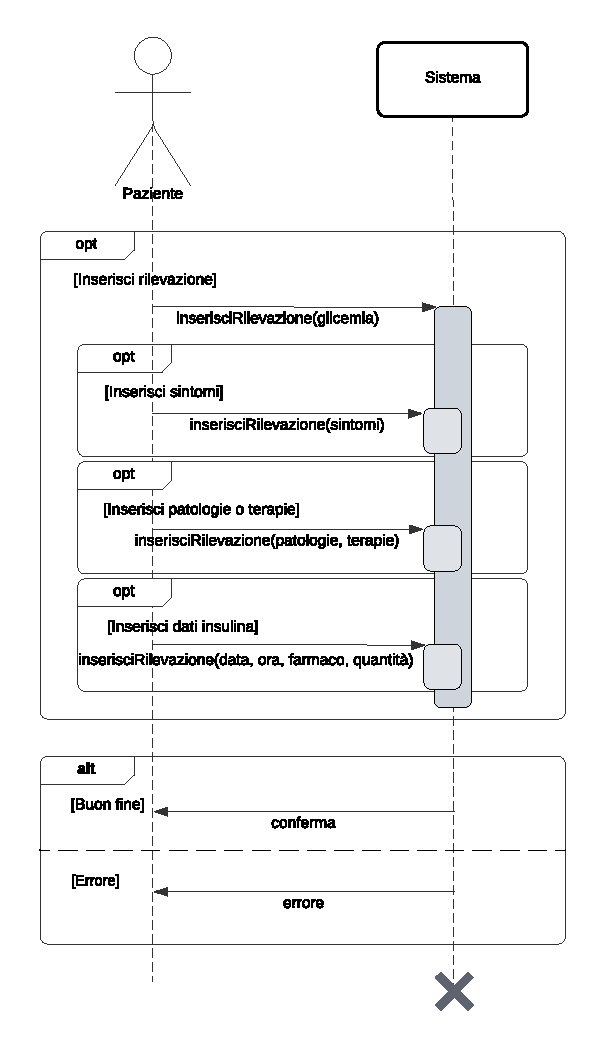
\includegraphics[width=0.7\textwidth]{sdPaziente}
  \caption{Sequence Diagram della rilevazione del paziente}
  \label{fig:sdPaziente}
\end{figure}

\subsection{Casi d'uso del medico}

\subsubsection{Visualizzare i dati del paziente}

\begin{mdframed}
  \textbf{Attore}: Medico\\
  \textbf{Precondizioni}: Il medico deve essere autenticato\\
  \textbf{Passi}: 
  \begin{enumerate}[nosep]
    \item Il medico accede alla sua area riservata
    \item Il medico può accedere alla lista dei pazienti
    \item Il medico può visualizzare i dati del paziente e lo storico delle rilevazioni
  \end{enumerate}
  \textbf{Postcondizioni}: nessuna
\end{mdframed}
\noindent
Il medico una volta che ha acceduto alla sua area riservata può visualizzare i dati di tutti i pazienti. 

\subsubsection{Modificare i dati del paziente}
\begin{mdframed}
  \textbf{Attore}: Medico\\
  \textbf{Precondizioni}: Il medico deve essere autenticato\\
  \textbf{Passi}: 
  \begin{enumerate}[nosep]
    \item Il medico accede alla sua area riservata
    \item Il medico accede alla lista dei pazienti
    \item Il medico seleziona il paziente che vuole gestire
    \item Il medico può decidere tra le seguenti opzioni:
      \begin{itemize}
        \item Aggiungere o modificare la terapia del paziente
        \item Aggiungere o modificare le note di un paziente
      \end{itemize}
    \item Il medico conferma le modifiche
    \item Il sistema aggiorna i dati del paziente
  \end{enumerate}
  \textbf{Postcondizioni}: La modifica è effettuata\\
  \textbf{Sequenza alternativa 1}: il medico può in qualunque momento decidere di annullare le modifiche
  e ritornare alla lista dei pazienti\\
  \textbf{Postcondizioni}: La modifica non è effettuata
\end{mdframed}
\noindent

\begin{figure}[H]
  \centering
  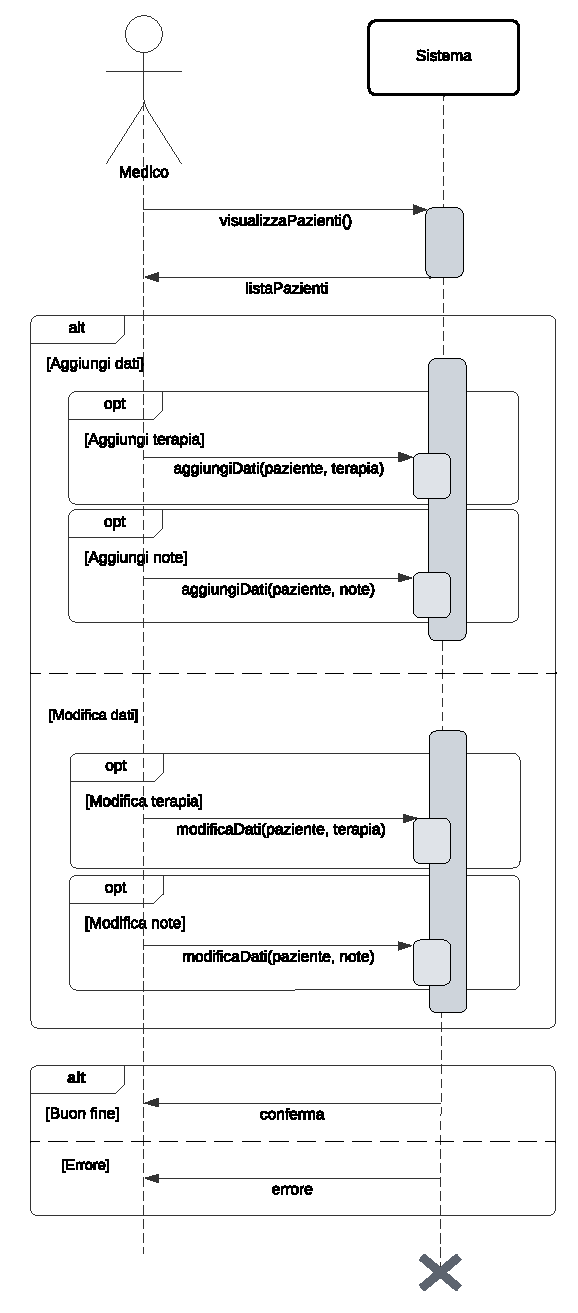
\includegraphics[width=0.65\textwidth]{sdMedico}
  \caption{Sequence Diagram del medico}
  \label{fig:sdMedico}
\end{figure}

\subsection{Ricezione delle notifiche}

Il paziente può ricevere notifiche dal sistema; se il pazienta si dimentica di assumere i farmaci
il sistema può inviare una notifica per ricordarglielo. 

\begin{mdframed}
  \textbf{Attore}: Paziente o Medico\\
  \textbf{Precondizioni}: Il paziente o medico deve essere autenticato\\
  \textbf{Passi}: 
  \begin{enumerate}[nosep]
    \item Il paziente o medico accede alla sua home page
    \item Il paziente o medico entra dentro la sezione delle notifiche
    \item  Il paziente o medico può visualizzare:
      \begin{itemize}
        \item  Notifiche già lette
        \item  Notifiche non lette
      \end{itemize}
  \end{enumerate}
  \textbf{Postcondizioni}: Se viene visualizzata una notifica, questa viene marcata come letta
\end{mdframed}


\begin{figure}[H]
  \centering
  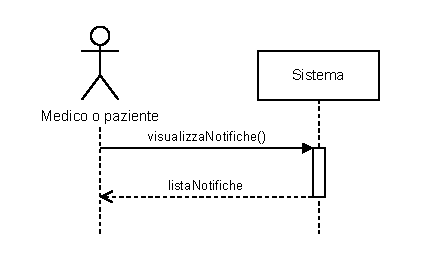
\includegraphics[width=0.7\textwidth]{sdNotifList.pdf}
  \caption{Sequence Diagram della notifica con lista}
  \label{fig:sdNotifList}
\end{figure}
\noindent
Il sistema invia delle notifiche ai seguenti attori:
\begin{itemize}
  \item \textbf{Al paziente}: per ricordargli di inserire i dati giornalieri
  \item \textbf{Al medico di riferimento del paziente}: per avvisare che il paziente  
    non ha seguito per più di tre giorni consecutivi le prescrizioni.
  \item \textbf{A tutti i medici}: per segnalare i pazienti che registrano
    livelli di glicemia sopra le soglie indicate.
\end{itemize}

\subsection{Casi d'uso dell'amministratore}

L'amministratore del servizio può gestire gli utenti del sistema. Si occupa di creare, modificare e cancellare
gli account dei pazienti e dei medici. Per agevolare l'aggiunta di utenti, ci si può registrare
tramite un form di registrazione (che specificherà il ruolo), ma l'amministratore deve comunque
approvare la registrazione per rendere l'utente attivo nel sistema.

\subsubsection{Gestione dell'utente}

\begin{mdframed}
  \textbf{Attore}: Amministratore\\
  \textbf{Precondizioni}: L'amministratore deve essere autenticato\\
  \textbf{Passi}: 
  \begin{enumerate}[nosep]
    \item L'amministratore accede alla sua area riservata
    \item L'amministratore visualizza la lista degli utenti
    \item L'amministratore può:
      \begin{itemize}
        \item  Creare un nuovo utente
        \item  Modificare un utente
        \item  Cancellare un utente
      \end{itemize}
  \end{enumerate}
  \textbf{Postcondizioni}: L'utente è creato, modificato o cancellato
\end{mdframed}

\subsubsection{Gestione delle richieste di registrazione}

\begin{mdframed}
  \textbf{Attore}: Amministratore\\
  \textbf{Precondizioni}: L'amministratore deve essere autenticato\\
  \textbf{Passi}: 
  \begin{enumerate}[nosep]
    \item L'amministratore accede alla sua area riservata
    \item L'amministratore visualizza la lista delle richieste
    \item Seleziona una richiesta di registrazione
    \item L'amministratore può:
      \begin{itemize}
        \item  Accettare una registrazione
        \item  Rifiutare una registrazione
      \end{itemize}
  \end{enumerate}
  \textbf{Postcondizioni}: L'utente è accettato o rifiutato
\end{mdframed}

\subsection{Visualizzazione della traccia dei medici}

Il sistema tiene traccia di ogni cambiamento o modifica che i medici effettuano sui pazienti, per 
ragioni di sicurezza.

\begin{itemize}
  \item L'amministratore può visualizzare questa traccia per verificare 
    che i medici non stiano effettuando operazioni non autorizzate.
  \item Il medico può visualizzare la traccia per verificare le operazioni effettuate
    precedentemente su un paziente da parte di altri medici
\end{itemize}

\begin{mdframed}
  \textbf{Attore}: Amministratore\\
  \textbf{Precondizioni}: L'amministratore deve essere autenticato\\
  \textbf{Passi}: 
  \begin{enumerate}[nosep]
    \item L'amministratore accede alla sua area riservata
    \item L'amministratore accede alla pagina di visualizzazione delle tracce 
  \end{enumerate}
  \textbf{Postcondizioni}: nessuna
\end{mdframed}

\begin{mdframed}
  \textbf{Attore}: Medico\\
  \textbf{Precondizioni}: Il medico deve essere autenticato\\
  \textbf{Passi}: 
  \begin{enumerate}[nosep]
    \item Il medico accede alla sua area riservata
    \item Il medico accede alla pagina di visualizzazione dei pazienti
    \item Il medico seleziona il paziente di cui vuole visualizzare la traccia
    \item Il medico accede alla schermata di visualizzazione della traccia dell'utente
  \end{enumerate}
  \textbf{Postcondizioni}: nessuna
\end{mdframed}


\subsection{Activity diagram}

Per semplicità non verrà rappresentato il fatto di poter ripetere le operazioni più volte,
ma si darà per scontato che l'utente possa tornare indietro e ripetere senza riavviare
il software. Vengono quindi rappresentate soltanto le singole attività di operazione.

Si da inoltre per scontato che per ogni attività (tranne la registrazione) l'utente sia
già autenticato e che non ci siano errori di autenticazione.

\subsubsection{Registrazione di un utente}

\begin{figure}[H]
  \begin{center}
    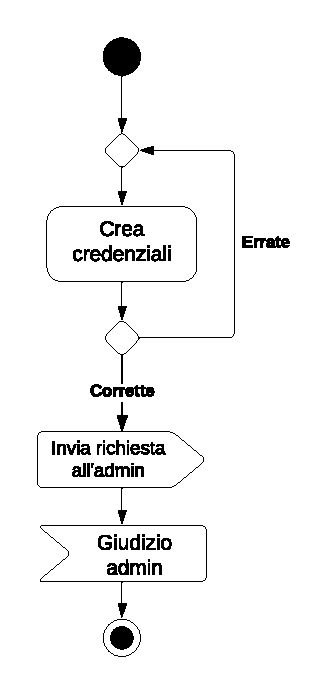
\includegraphics[width=0.4\textwidth]{adRegistrazione}
  \end{center}
  \caption{Activity diagram della registrazione di un utente}
  \label{fig:adRegistrazione}
\end{figure}

\subsubsection{Attività del paziente}

\begin{figure}[H]
  \begin{center}
    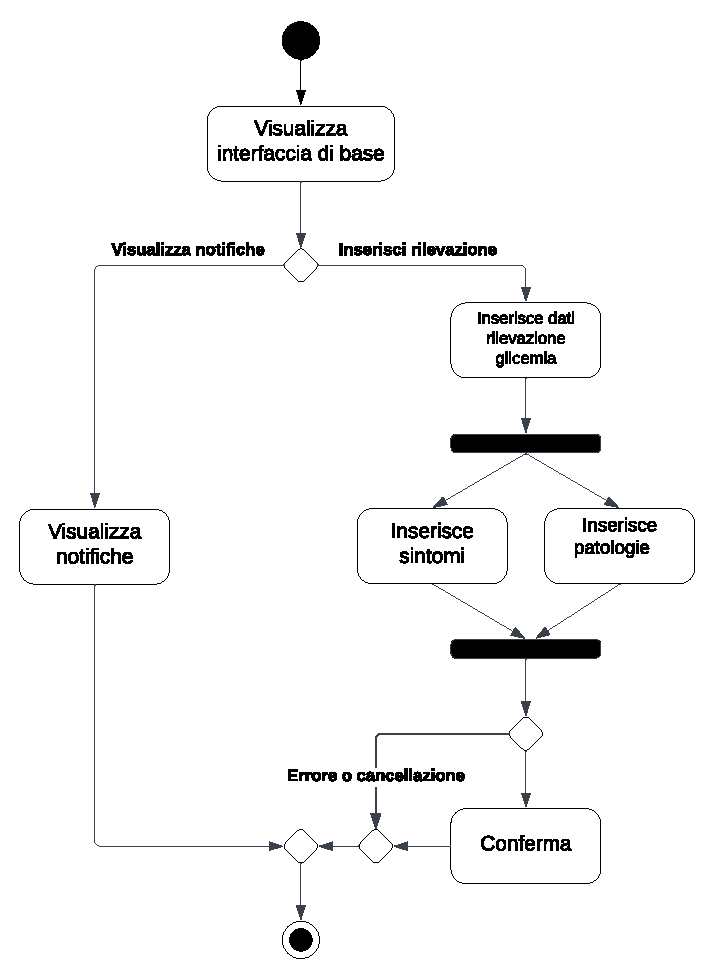
\includegraphics[width=0.8\textwidth]{adPaziente}
  \end{center}
  \caption{Activity diagram del paziente}
  \label{fig:adPaziente}
\end{figure}

\subsubsection{Attività del medico}

\begin{figure}[H]
  \begin{center}
    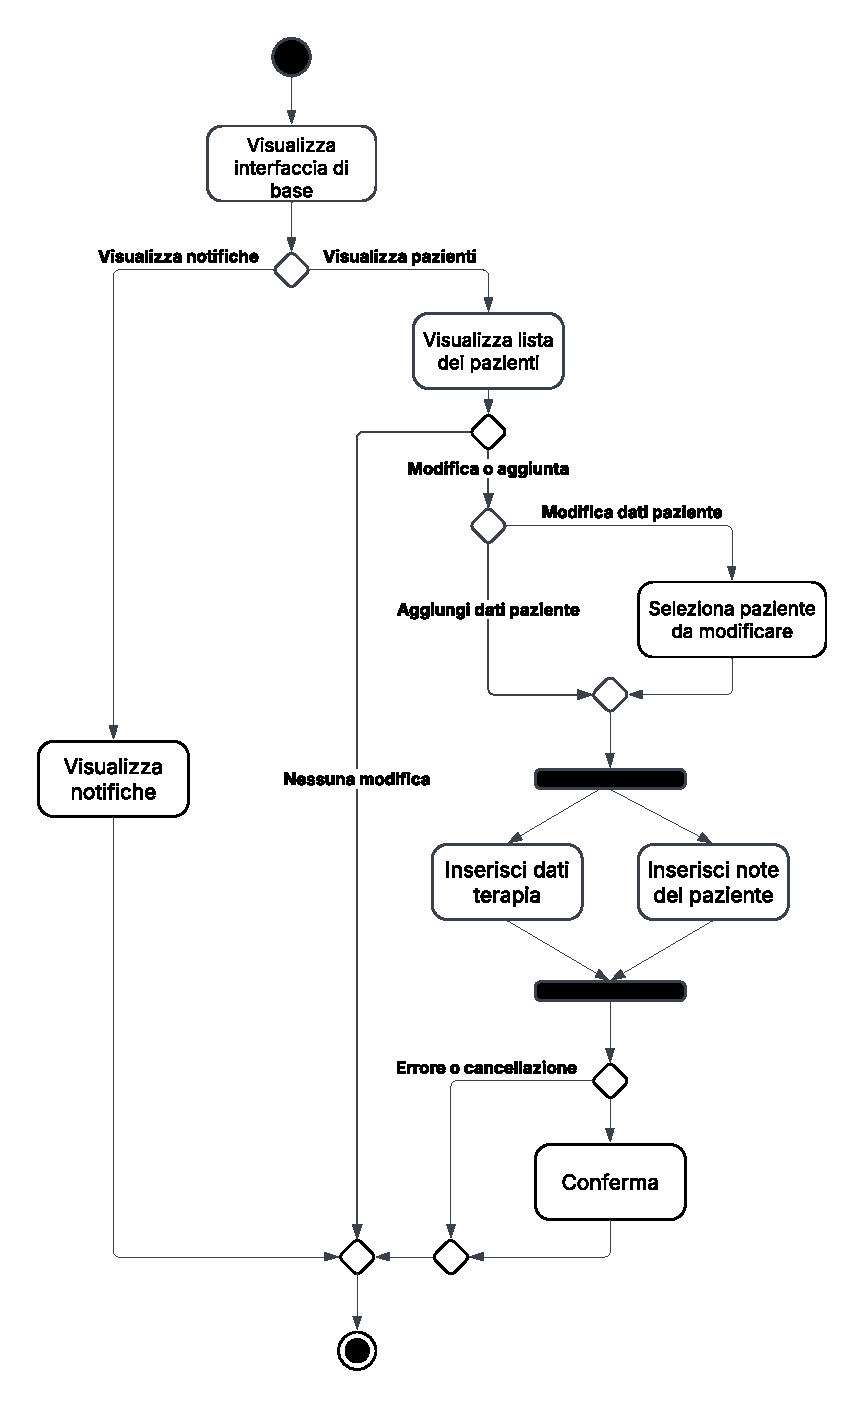
\includegraphics[width=0.9\textwidth]{adMedico}
  \end{center}
  \caption{Activity diagram del medico}
  \label{fig:adMedico}
\end{figure}

\subsubsection{Attività dell'amministratore}

\begin{figure}[H]
  \begin{center}
    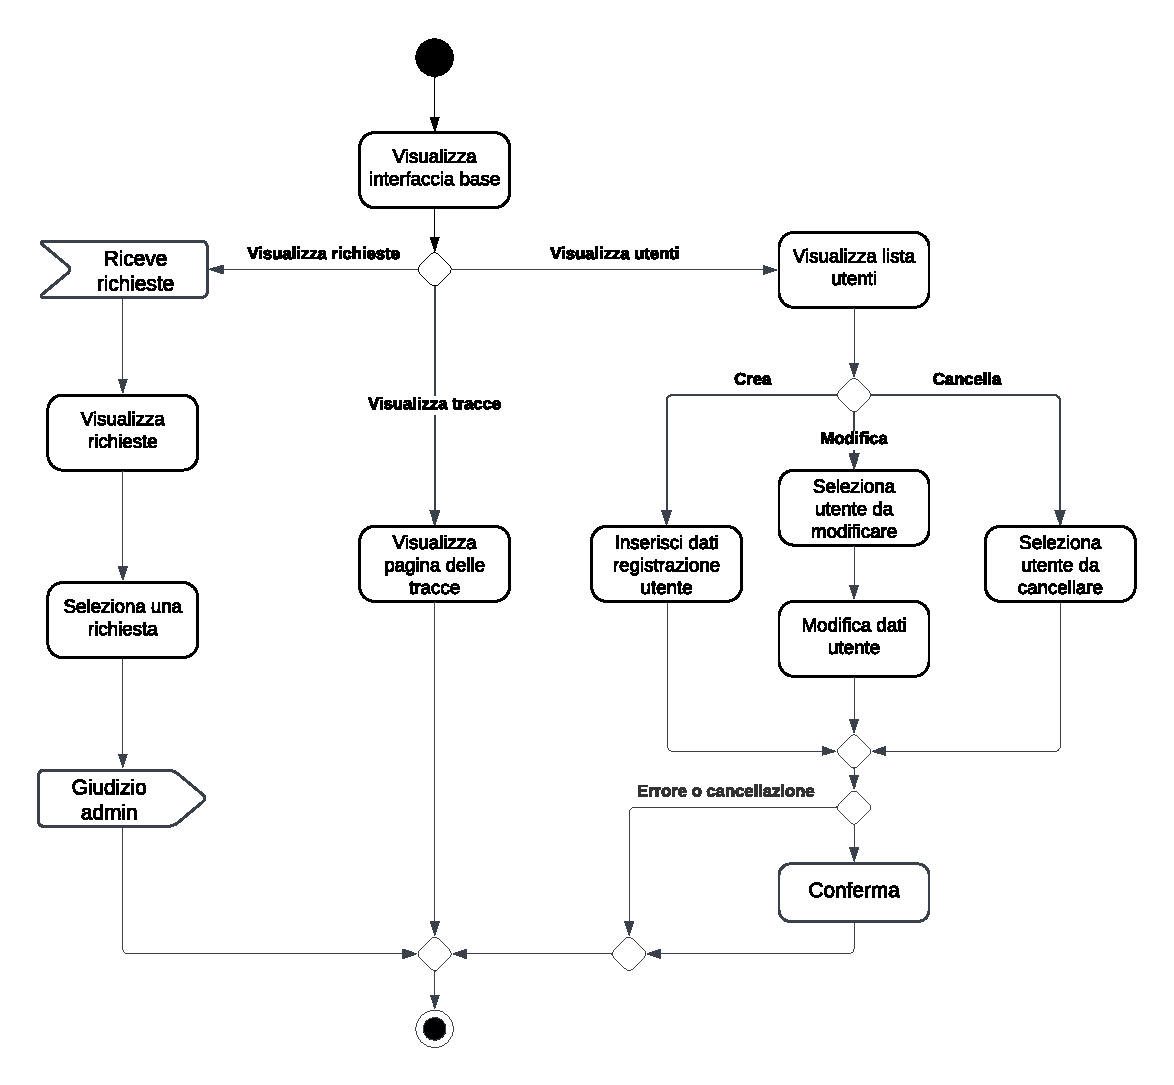
\includegraphics[width=1\textwidth]{adAmministratore}
  \end{center}
  \caption{Activity diagram dell'amministratore}
  \label{fig:adAmministratore}
\end{figure}

\section{Sviluppo}

\subsection{Processo di sviluppo}

Il processo di sviluppo del software è stato realizzato seguendo il modello \textit{Agile} con metodologia \textit{Scrum}.
Il team è composto da due sviluppatori, che hanno lavorato in parallelo su diverse funzionalità del software.
Lo Scrum ci ha permesso di organizzare il lavoro in sprint precisi, durante i quali abbiamo
sviluppato le funzionalità richieste, testandole e integrandole nel software. 
Gli sprint venivano pianificati in base alle funzionalità da implementare e alle priorità stabilite all'inizio,
facendo una scrematura delle funzionalità da implementare in base al tempo a disposizione. 
Alla fine di ogni sprint, abbiamo effettuato una revisione del lavoro svolto, testando le funzionalità implementate e correggendo eventuali bug.
\textit{Product Backlog} e \textit{Sprint Backlog} non sono nient'altro che una lista di "to-do" task che bisogna affrontare per la scelta delle funzionalità da implementare
e su come implementarle rispettivamente. Tuttavia non vi è un \textit{Scrum Master} in quanto il team è composto da due persone e non vi è la necessità di avere una figura che coordini il lavoro.
\begin{figure}[H]
  \begin{center}
    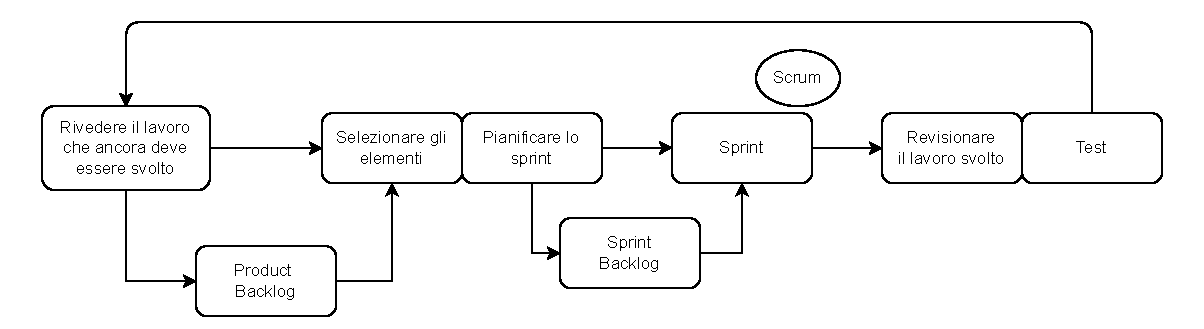
\includegraphics[width=1\textwidth]{adProcessodiSviluppo.pdf}
  \end{center}
  \caption{Diagramma del processo di sviluppo}
  \label{fig:adProcessodiSviluppo}
\end{figure}
\noindent
Prima di cominciare il ciclo di Scrum però, è stata effettuata una fase di \textit{analisi dei requisiti}, dove tutto il team di Scrum si è unito per 
analizzare le specifiche del progetto e poi sono stati definiti i casi d'uso (vedi figura \ref{fig:usecase}).
Man mano che venivano implementate le classi e le funzionalità, veniva aggiornata la documentazione per assicurarci che sia tutto coerente e che non ci fossero errori.
Per la gestione del codice sorgente, è stato utilizzato \textit{Git} come sistema di versionamento, con un repository su \textit{GitHub} per facilitare la collaborazione tra i membri del team.
Abbiamo utilizzato anche \textit{Github Planner} per tenere traccia delle attività da svolgere e dello stato di avanzamento del progetto.

\begin{figure}[H]
  \begin{center}
    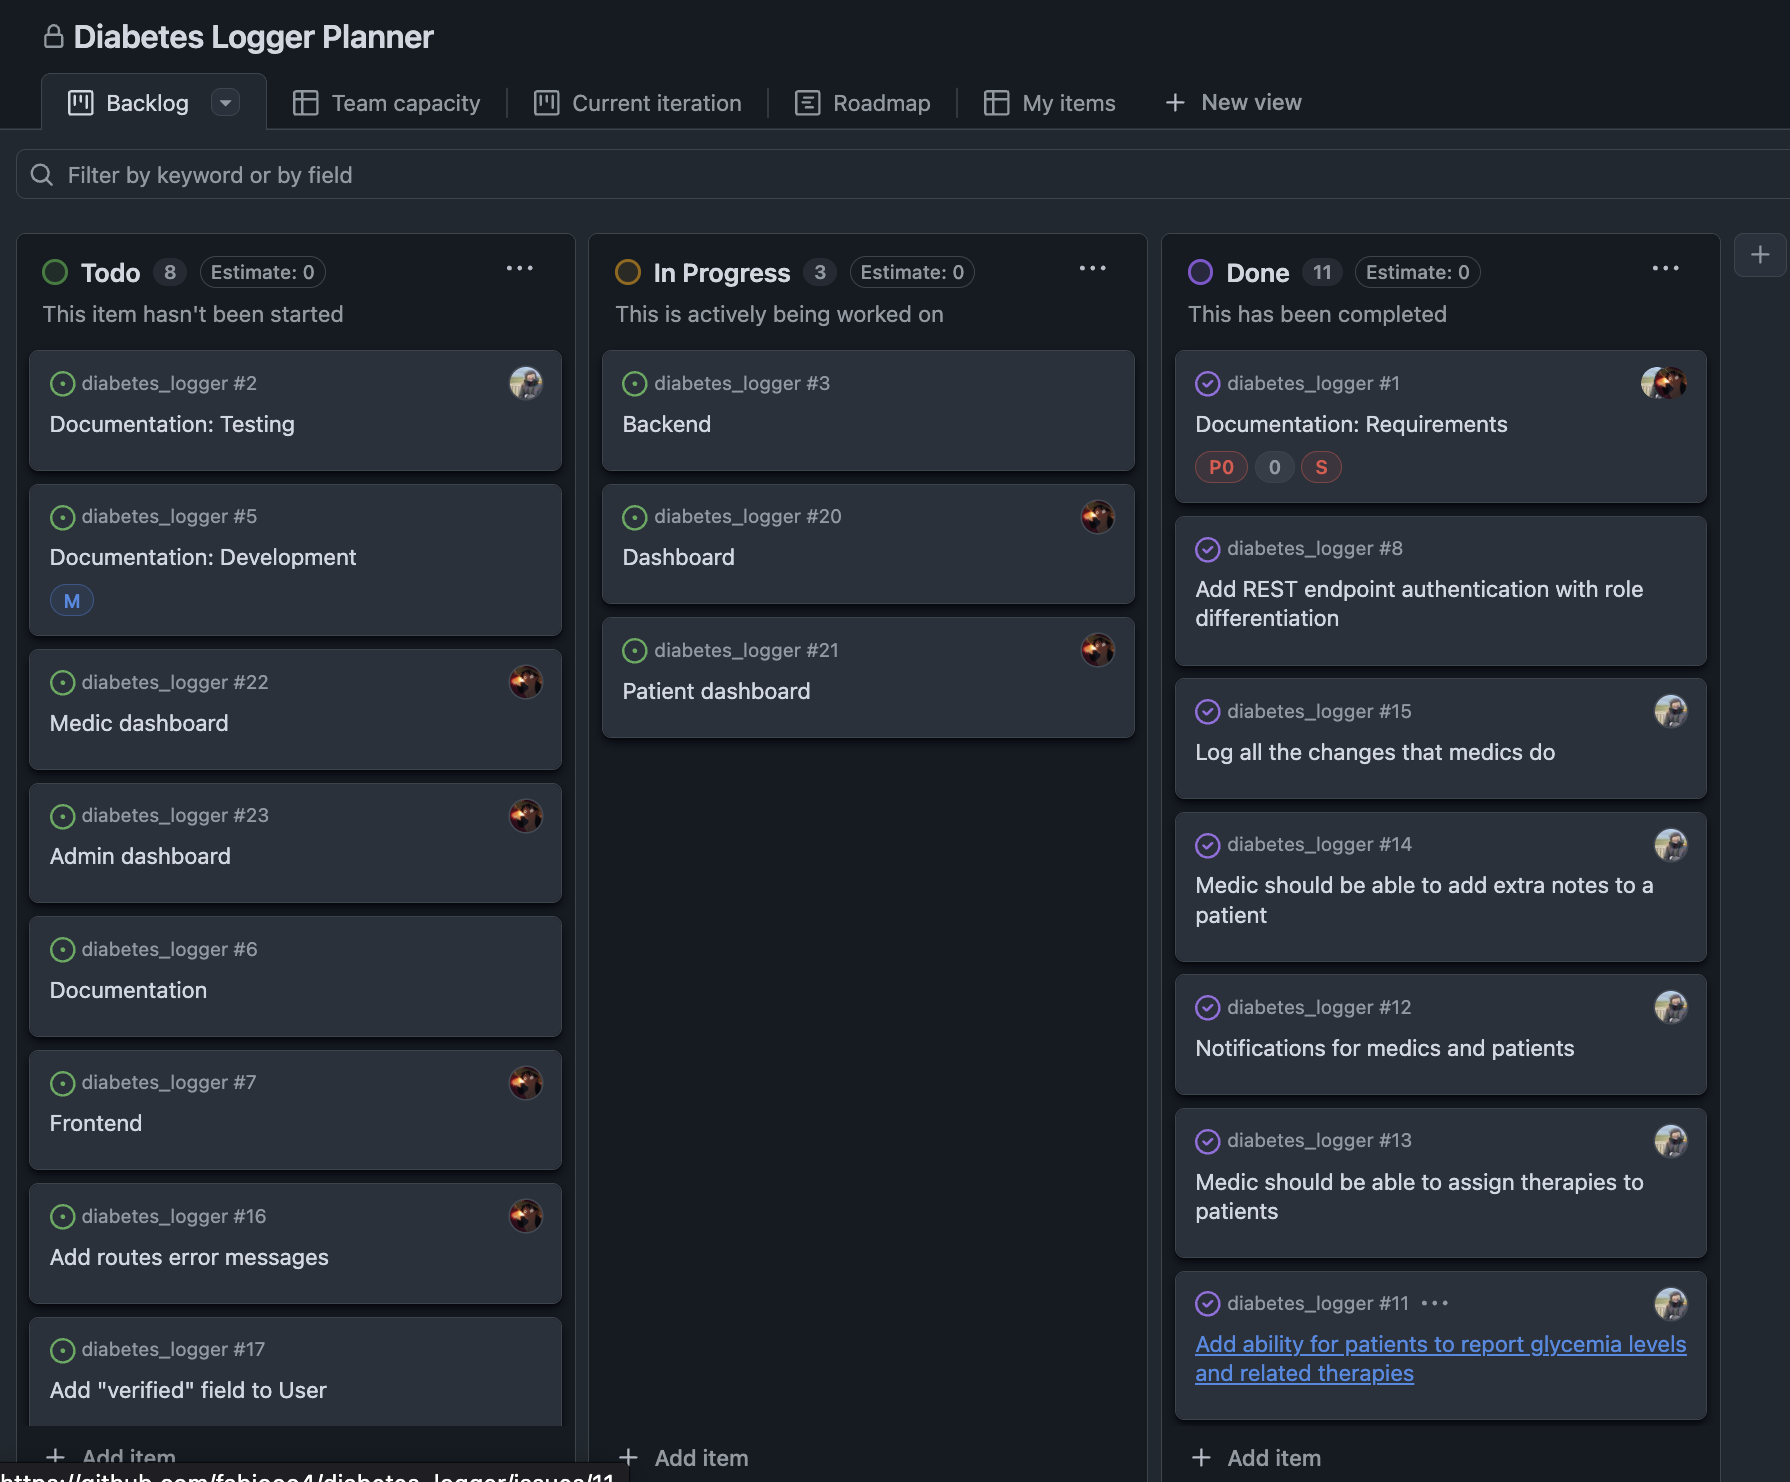
\includegraphics[width=0.9\textwidth]{githubPlanner.png}
  \end{center}
  \caption{Github Planner del progetto} 
  \label{fig:githubPlanner}
\end{figure}

\subsection{Progettazione e pattern architetturali usati}

Il software è stato progettato seguendo un’architettura di tipo \textit{Client-Server}, 
ispirata al pattern \textit{Model-View-Controller (MVC)}, 
seppur con alcune differenze rispetto alla sua implementazione classica.
 In particolare, il sistema è suddiviso in due componenti principali:

\begin{itemize}
  \item \textbf{Client (View)}: responsabile dell’interfaccia utente e dell’interazione con 
  l’utente finale. È implementato tramite \textit{SvelteKit}, un framework moderno per applicazioni web. 
  Il client si occupa esclusivamente della presentazione e invia richieste HTTP al server per ottenere 
  o modificare i dati.
  \item \textbf{Server (Model + Controller)}: realizzato con \textit{Spring Boot}, gestisce sia 
  la logica di business (Model) che il controllo delle richieste (Controller). Il server espone delle 
  Web API che il client può invocare.
  \begin{itemize}
    \item \textbf{Model}: rappresenta le entità principali del sistema, come utenti, pazienti, medici, 
    rilevazioni, notifiche e il change log.
    \item \textbf{Controller}: gestisce le richieste provenienti dal client, delega 
    le operazioni al Model e restituisce le risposte appropriate.
  \end{itemize}
\end{itemize}
\noindent
Questa separazione ha garantito una buona modularità del sistema, migliorando la manutenibilità e 
facilitando l’evoluzione indipendente del frontend e del backend.
Nel prosieguo della documentazione verrà analizzato in dettaglio il \textbf{Model}, 
in quanto contiene le classi che rappresentano gli attori del sistema e le loro interazioni.


\begin{figure}[H]
  \begin{center}
    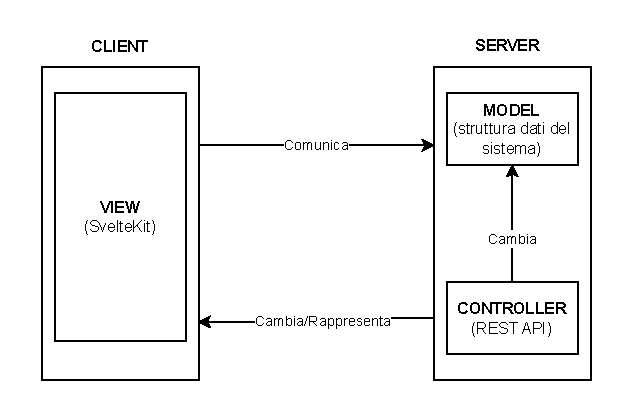
\includegraphics[width=0.9\textwidth]{ClientServerMVC.pdf}
  \end{center}
  \caption{Architettura Client-Server ispirata al pattern MVC} 
  \label{fig:mvc}
\end{figure}
\noindent
Seguono i diagrammi UML delle classi del Model e del Controllore, che rappresentano le entità principali del software e le loro relazioni.
\begin{figure}[H]
  \begin{center}
    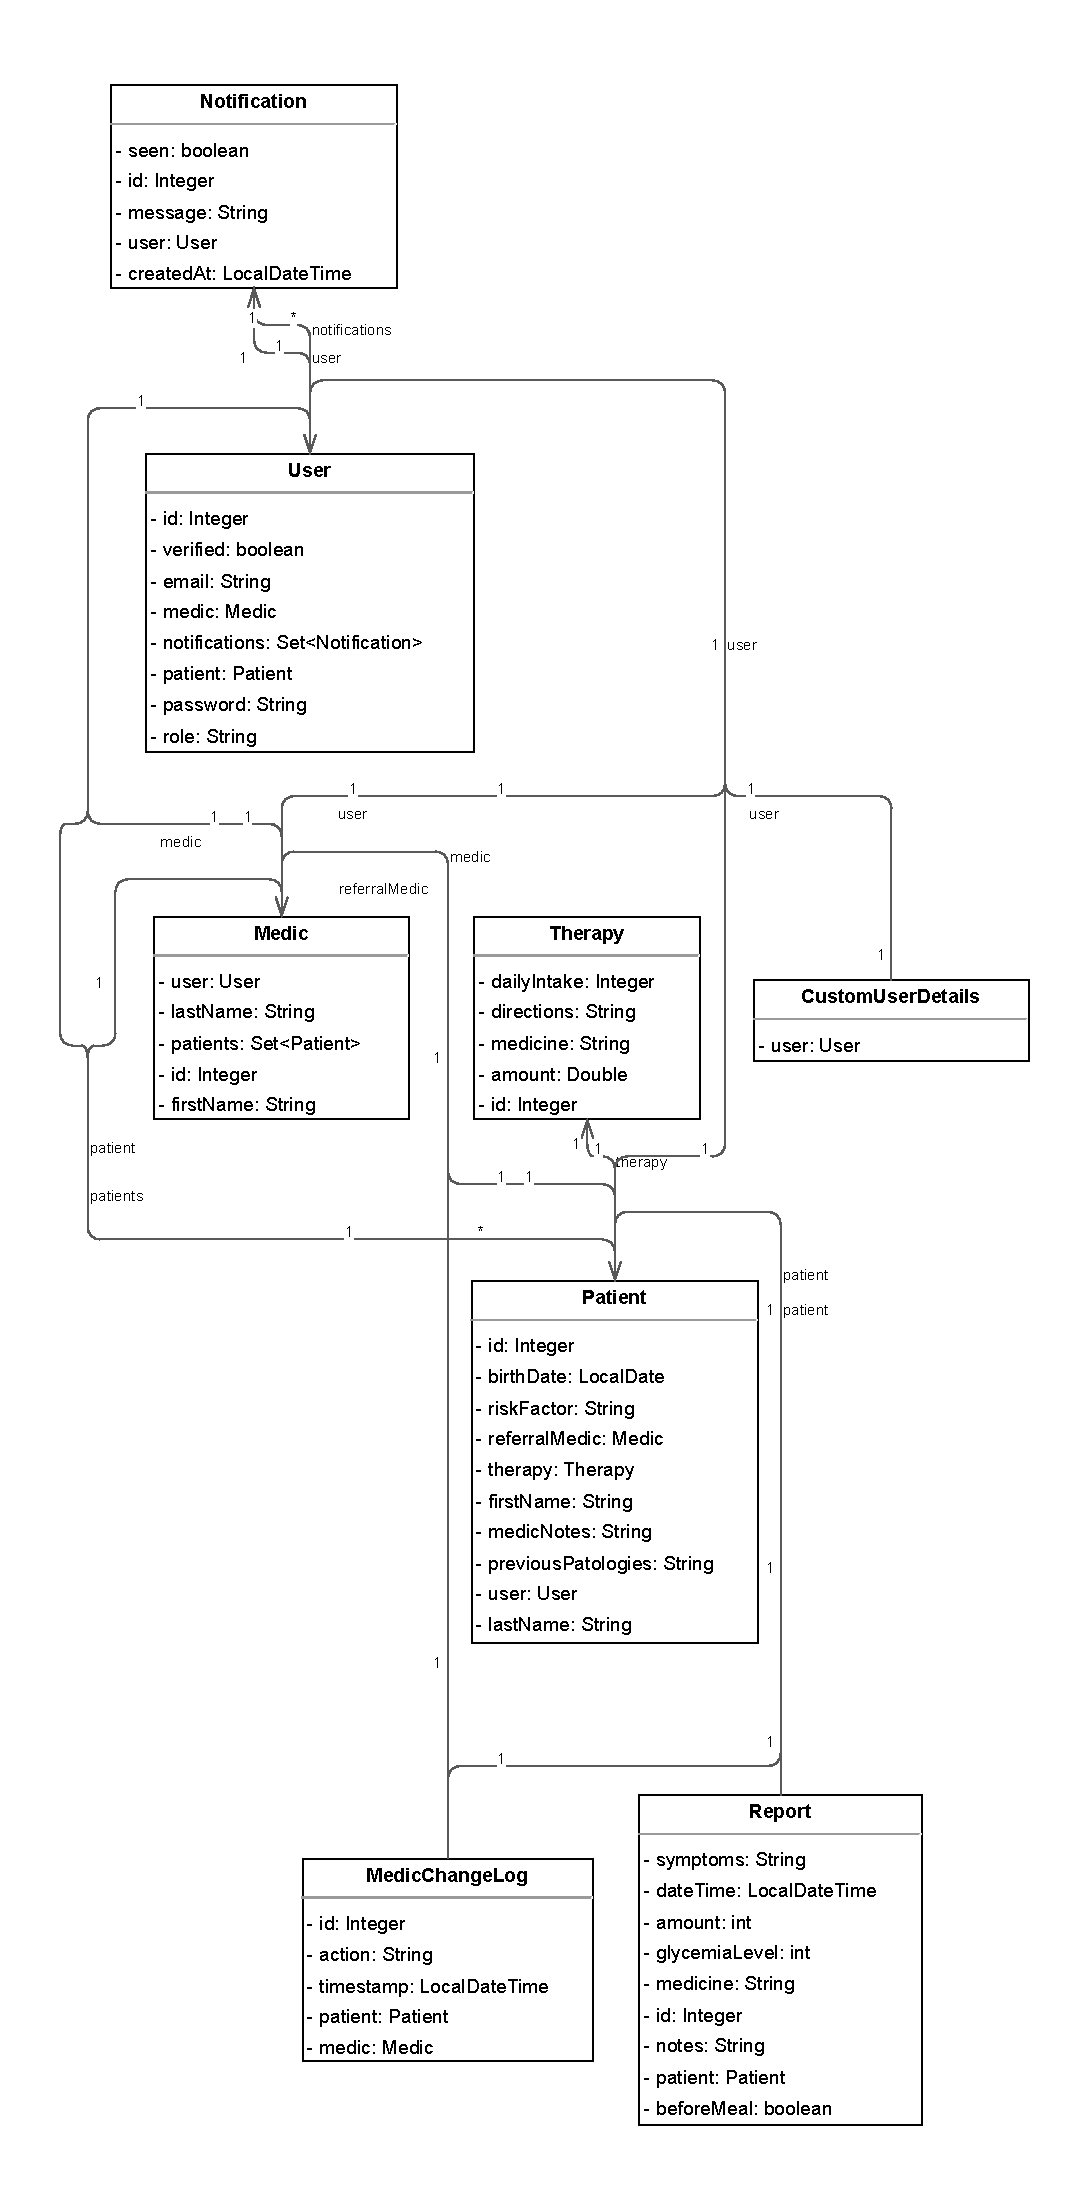
\includegraphics[width=0.9\textwidth]{umlModel.pdf}
  \end{center}
  \caption{Diagramma UML delle classi del Model con relativi endpoints} 
\end{figure}
\noindent
\begin{figure}[H]
  \begin{center}
    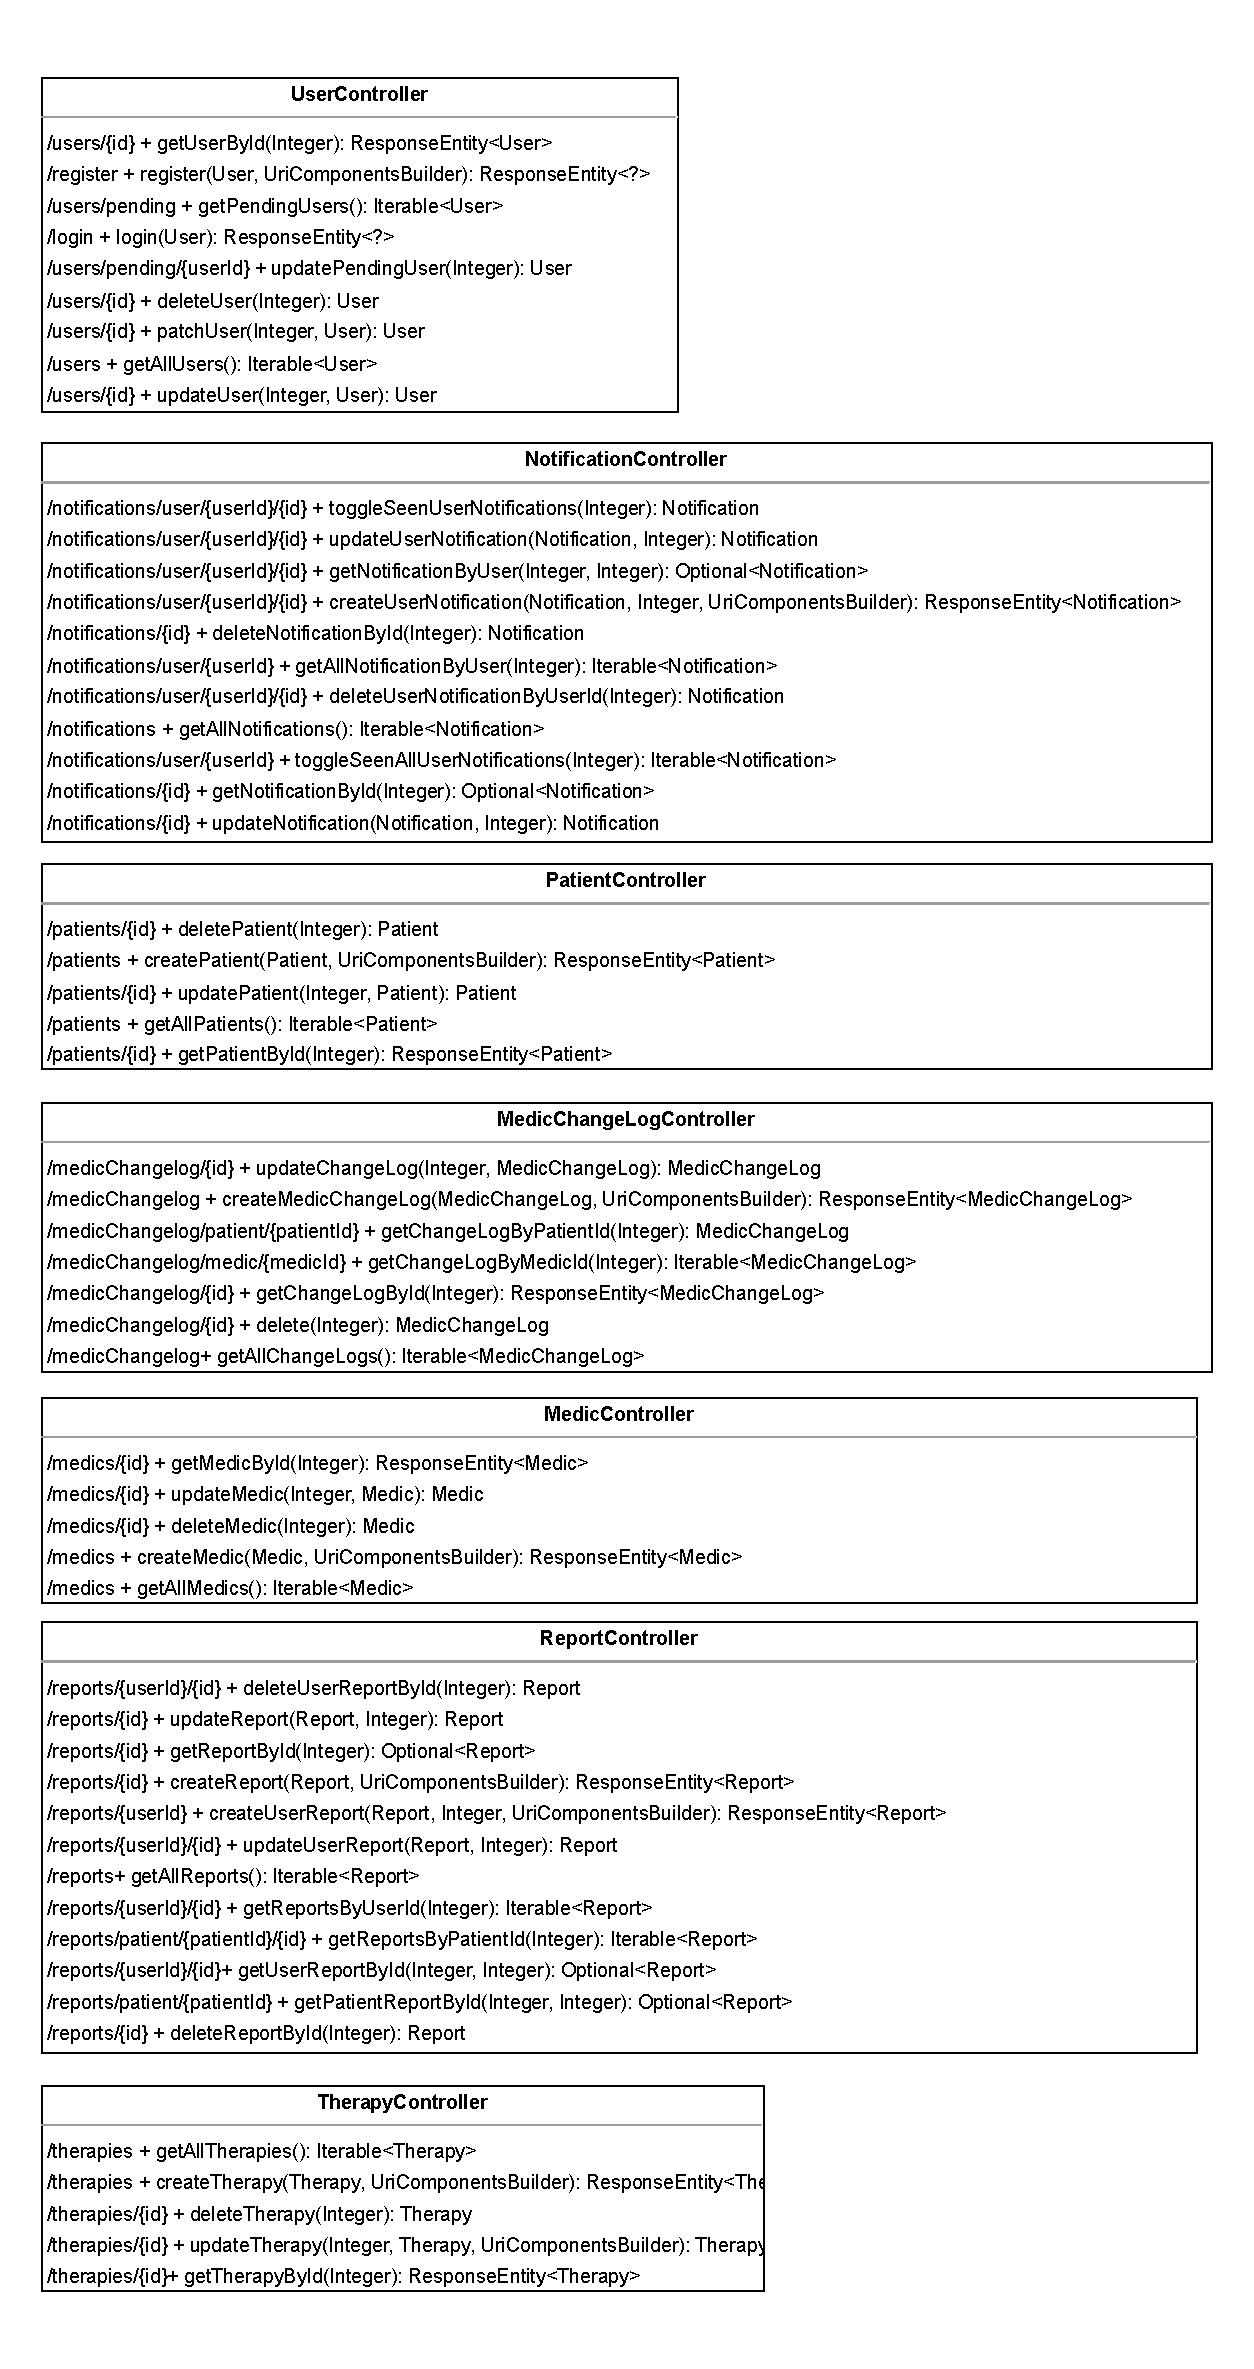
\includegraphics[width=1\textwidth]{uml.pdf}
  \end{center}
  \caption{Classi UML dei Controller} 
  \label{fig:controller}
\end{figure}
\noindent

\subsection{Comunicazione e gestione delle richieste}

Per gestire la comunicazione tra le componenti del software sono state effettuate le seguenti scelte:
\begin{itemize}
  \item Per la comunicazione tra il Model e il Controller, sono stati utilizzati i \textit{Repository} di Spring Boot, 
  che permettono di interagire con il database in modo semplice e veloce. Dopodiché abbiamo implementato
  i \textit{Service} che contengono la logica di business e le operazioni da effettuare sui dati. Abbiamo creato
  un interfaccia \textit{CrudService} che contiene i metodi CRUD (Create, Read, Update, Delete) che ogni servizio implementa.
  \item Per la comunicazione tra il Controller e la View, sono stati utilizzati i \textit{REST Controller} di Spring Boot, 
  che permettono di gestire le richieste HTTP e di restituire le risposte in formato JSON.
  \item Per la comunicazione tra il Model e la View in realtà, non c'è una comunicazione diretta, ma il Controller
  si occupa di prendere i dati dal Model e passarli alla View tramite le richieste HTTP. Questo ci permette 
  di poter decidere quando vogliamo di cambiare modalità di View senza dover modificare il Model.
\end{itemize}

\subsection{Implementazione e design dei pattern usati}

\subsubsection{Generalità}

Ora andremo a vedere quali sono i pattern implementati nel software e come sono stati utilizzati.

\begin{itemize}
  \item I \textbf{pattern iterator} sono stati utilizzati per iterare sulle liste di tutti i nostri modelli, proprietà intrinseca
  di Java. 
  \item È stato utilizzato molteplici volte il \textbf{pattern Observer} grazie alle dipendenze fornite da Spring Boot 
  tramite annotazioni come \textit{@ManyToOne} e \textit{@OneToMany}: quindi quando un oggetto viene modificato,
  tutti gli oggetti che dipendono da esso vengono notificati e aggiornati automaticamente.
  \item Per gestire l'autenticazione e la sicurezza degli endpoints, è stato utilizzato il \textbf{pattern Security} di Spring Boot,
  che permette di gestire l'autenticazione e l'autorizzazione degli utenti. Tuttavia, in concomitanza abbiamo dovuto usare 
  il \textbf{pattern Adapter} per adattare le nostre classi di autenticazione a quelle di Spring Boot e alle nostre esigenze
  (più approfondimenti sul pattern adapter nella sezione \textit{Autenticazione e autorizzazione}).
  \item Il \textbf{pattern Factory Method} è stato utilizzato per comporre le classi del Model come le repository
  e tutto il service layer (che implementano l'interfaccia \textit{CrudService}) e implementano i loro metodi in base 
  alle esigenze del progetto.
  \item A sua volta, all'interno della configurazione per la sicurezza, è stato utilizzato il \textbf{Filter Pattern}
  dove una serie di filtri (autenticazione, autorizzazione, ecc.) processano la richiesta in sequenza.
\end{itemize}

\subsubsection{Autenticazione e autorizzazione}

Per gestire l'autenticazione e l'autorizzazione degli utenti, è stato utilizzata la libreria \textit{Spring Security}, che permette di gestire
l'autenticazione e l'autorizzazione degli utenti. 

\begin{figure}[H]
  \begin{center}
    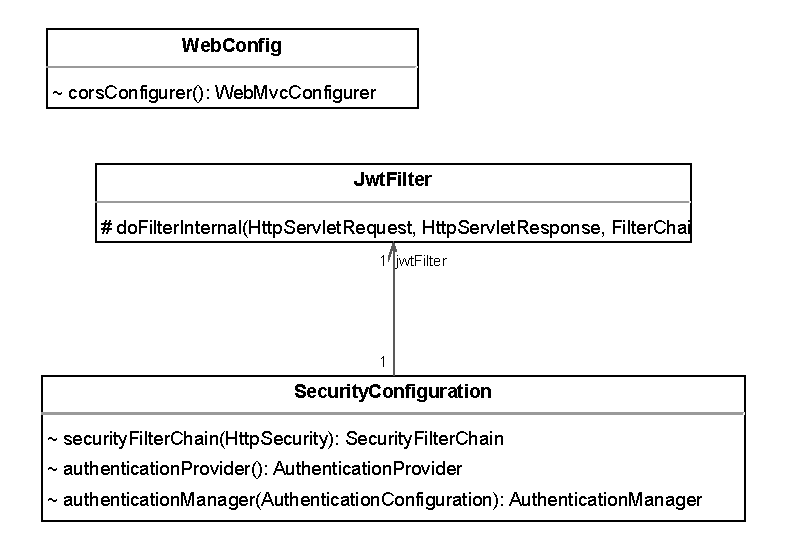
\includegraphics[width=1\textwidth]{config.pdf}
  \end{center}
  \caption{Classi UML della configurazione della sicurezza} 
\end{figure}
\noindent
Di seguito sono riportate le classi principali che compongono la configurazione della sicurezza:
\begin{itemize}
  \item La classe \textbf{WebConfig} si occupa di configurare le impostazioni di sicurezza del web, come i CORS e le risorse statiche.
  Nel nostro caso ci permette di effettuare richieste dallo stesso IP del server, ma su porte diverse (per esempio, il frontend).
  \item La classe \textbf{JwtFilter} si occupa di filtrare le richieste HTTP e di verificare se l'utente è autenticato tramite un token JWT.
  I token JWT (JSON Web Token) sono un modo per rappresentare le informazioni di autenticazione in modo sicuro e compatto.
  In poche parole estraiamo il token JWT dalla richiesta HTTP e lo verifichiamo per vedere se è valido.
  \item La classe \textbf{SecurityConfiguration} è stata implementata usando il \textbf{builder Pattern} e si occupa di configurare la sicurezza del progetto,
  infatti possiamo definire una serie di filtri che processano la richiesta in sequenza.
  Quindi, nella funzione \textit{securityFilterChain} definiamo i filtri che vogliamo utilizzare, come il filtro di autenticazione e il filtro di autorizzazione.
  Questo ci permette di definire i permessi di ogni ruolo, quindi per esempio, i pazienti possono accedere solo alle loro informazioni, i medici possono accedere alle informazioni dei pazienti 
  e l'amministratore può accedere a tutte le informazioni (vedere \ref{fig:usecase}).
\end{itemize}
Stiliamo ora un breve elenco degli endpoints a cui possono accedere i vari ruoli:
\begin{itemize}
  \item Admin:
  \begin{itemize}
    \item \textbf{GET+POST+PUT+DELETE/**}
  \end{itemize}

  \item Pazienti:
  \begin{itemize}
    \item UsersController: 
    \begin{itemize}
      \item \textbf{GET+PATCH /users/\{loggedId\}}
    \end{itemize}
    \item ReportsController: \begin{itemize}
      \item \textbf{GET+POST+PUT+DELETE /reports/user/\{loggedId\}/\{id\}}
      \item \textbf{GET /reports/user/\{loggedId\}}
    \end{itemize}
    \item NotificationsController: 
    \begin{itemize}
      \item \textbf{GET+DELETE+PATCH /notifications/user/\{userId\}/\{loggedId\}}
      \item \textbf{GET+PATCH /notifications/user/\{userId\}}
    \end{itemize}
  \end{itemize}

  \item Medici:
  \begin{itemize}
    \item UsersController:
    \begin{itemize}
      \item \textbf{GET+PATCH /users/\{loggedId\}} 
    \end{itemize}
    \item ReportsController:
    \begin{itemize}
      \item \textbf{GET /reports/\{anyUserId\}}
      \item \textbf{GET /reports/patient/\{anyPatientId\}}
      \item \textbf{GET /reports}
    \end{itemize}
    \item NotificationsController:
    \begin{itemize}
      \item \textbf{GET+DELETE+PATCH /notifications/user/\{userId\}/\{loggedId\}}
      \item \textbf{GET+PATCH /notifications/user/\{userId\}}
    \end{itemize}
    \item TherapiesController:
    \begin{itemize}
      \item \textbf{GET+POST /therapies}
      \item \textbf{GET+PUT /therapies/\{userId\}}
    \end{itemize}
    \item PatientsController:
    \begin{itemize}
      \item \textbf{GET /patients}
      \item \textbf{GET /patients/\{anyPatientId\}}
      \item \textbf{PUT /patients/medic/\{medicId\}/\{anyPatientId\}}
    \end{itemize}
    \item MedicChangeLogController:
    \begin{itemize}
      \item \textbf{GET /medicChangeLog/patient/\{patientId\}}
    \end{itemize}
  \end{itemize}
\end{itemize}
\noindent
I seguenti termini fanno riferimento a identificatori variabili all'interno degli endpoints
e sono defiiniti nel modo seguente:
\begin{itemize}
  \item \textbf{loggedId}: è l'id dell'utente che è autenticato
  con un JWT token valido.
  \item \textbf{anyUserId}: è l'id di un qualsiasi utente
  \item \textbf{anyPatientId}: è l'id di un qualsiasi paziente, quindi può 
  essere un paziente che non è l'utente autenticato
  \item \textbf{userId}: è l'id di un utente qualsiasi, può essere anche un utente non autenticato
\end{itemize}

\subsubsection{Model: repository e service layer}

Il nostro Model è composto da diverse classi che rappresentano gli attori del sistema e le loro interazioni.
La nostra logica di business è separata in \textit{layer}  contenuti dentro \textbf{package} 
per garantire una buona organizzazione del codice e una facile navigazione, insieme
ad un controllo degli errori più semplice.
Questi layer sono:
\begin{itemize}
  \item \textbf{Model}: è il package principale perché contiene tutte le definizioni delle entità del sistema, come \textit{User}, \textit{Patient}, \textit{Medic}, \textit{MedicChangeLog}, \textit{Report}, \textit{Notification} e \textit{Therapy}.
  \item \textbf{Repository}: è il package che contiene le interfacce dei repository, che sono utilizzate per interagire con il database. 
  Abbiamo utilizzato JPA (Jakarta Persistance API) Repository di Spring Boot, che ci ha permesso di immagazinare e ottenere i dati da un 
  database relazionale. 
  Le interfacce dei repository estendono \textit{JpaRepository} e forniscono i metodi per effettuare le operazioni CRUD sui dati.
  \item \textbf{Service}: è il package che contiene le classi dei servizi, che sono utilizzate per gestire la logica di business del software. 
  Infatti, le classi dei servizi implementano l'interfaccia \textit{CrudService} che contiene i metodi CRUD che ogni servizio deve implementare.
  I servizi astraggono e ampliano le funzionalità della repository.
  I servizi sono utilizzati dai controller per gestire le richieste degli utenti e interagire con i repository.
\end{itemize}
Il controller (vedi figura \ref{fig:controller}) come già stato detto, utilizza il Model per 
gestire le richieste degli utenti e interagire con i dati. 
Seguono sequence diagram di alcune interazioni e dinamiche importanti del software:
\begin{figure}[H]
  \begin{center}
    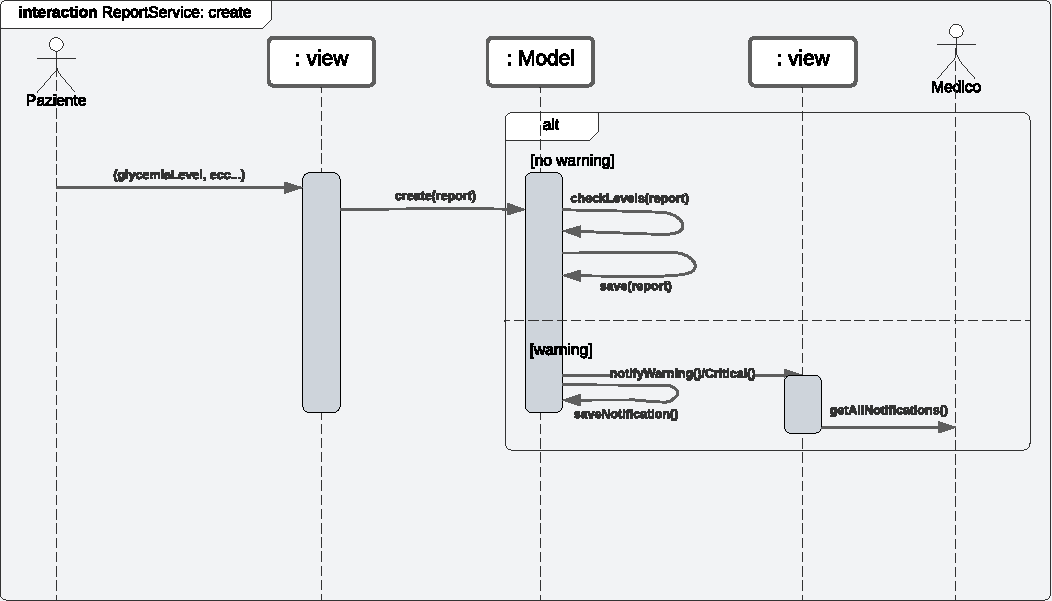
\includegraphics[width=1\textwidth]{sdReportCreate.pdf}
  \end{center}
  \caption{Sequence Diagram della creazione di un report + makeNotification} 
\end{figure}
\noindent

\begin{figure}[H]
  \begin{center}
    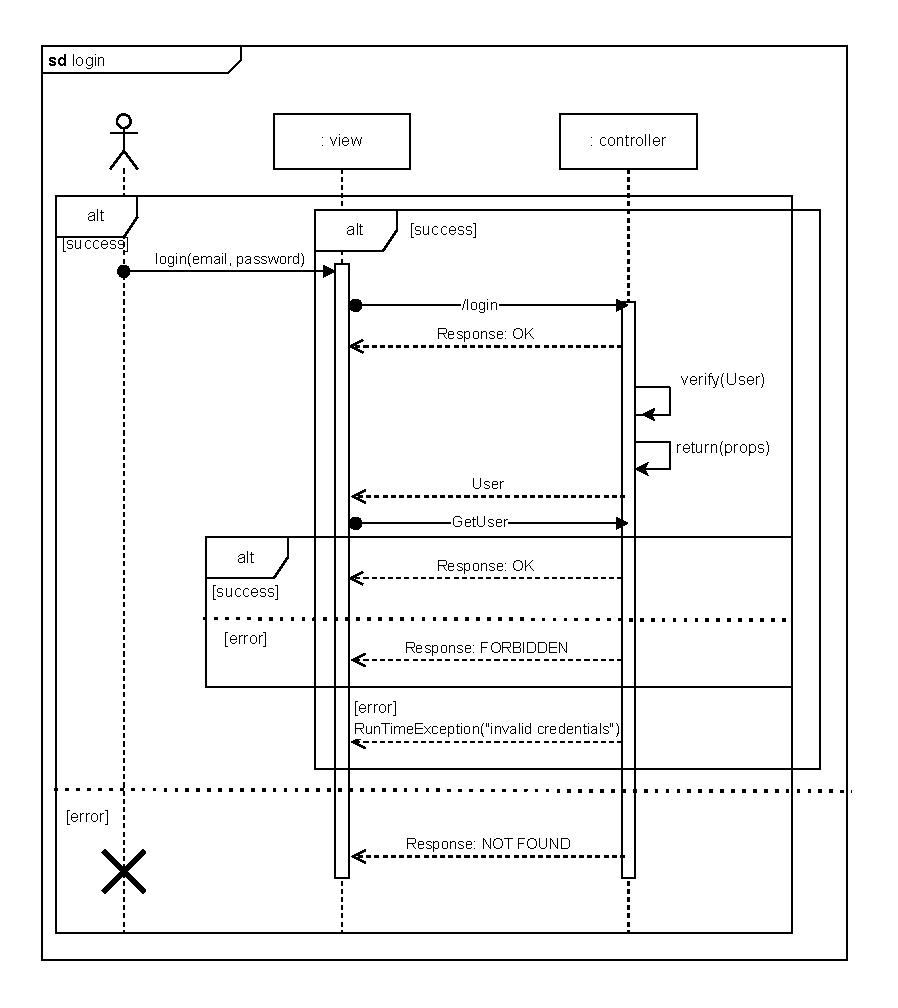
\includegraphics[width=1\textwidth]{login.pdf}
  \end{center}
  \caption{Sequence Diagram di un login e della creazione di un token JWT (props)}  
\end{figure}
\noindent

\begin{figure}[H]
  \begin{center}
    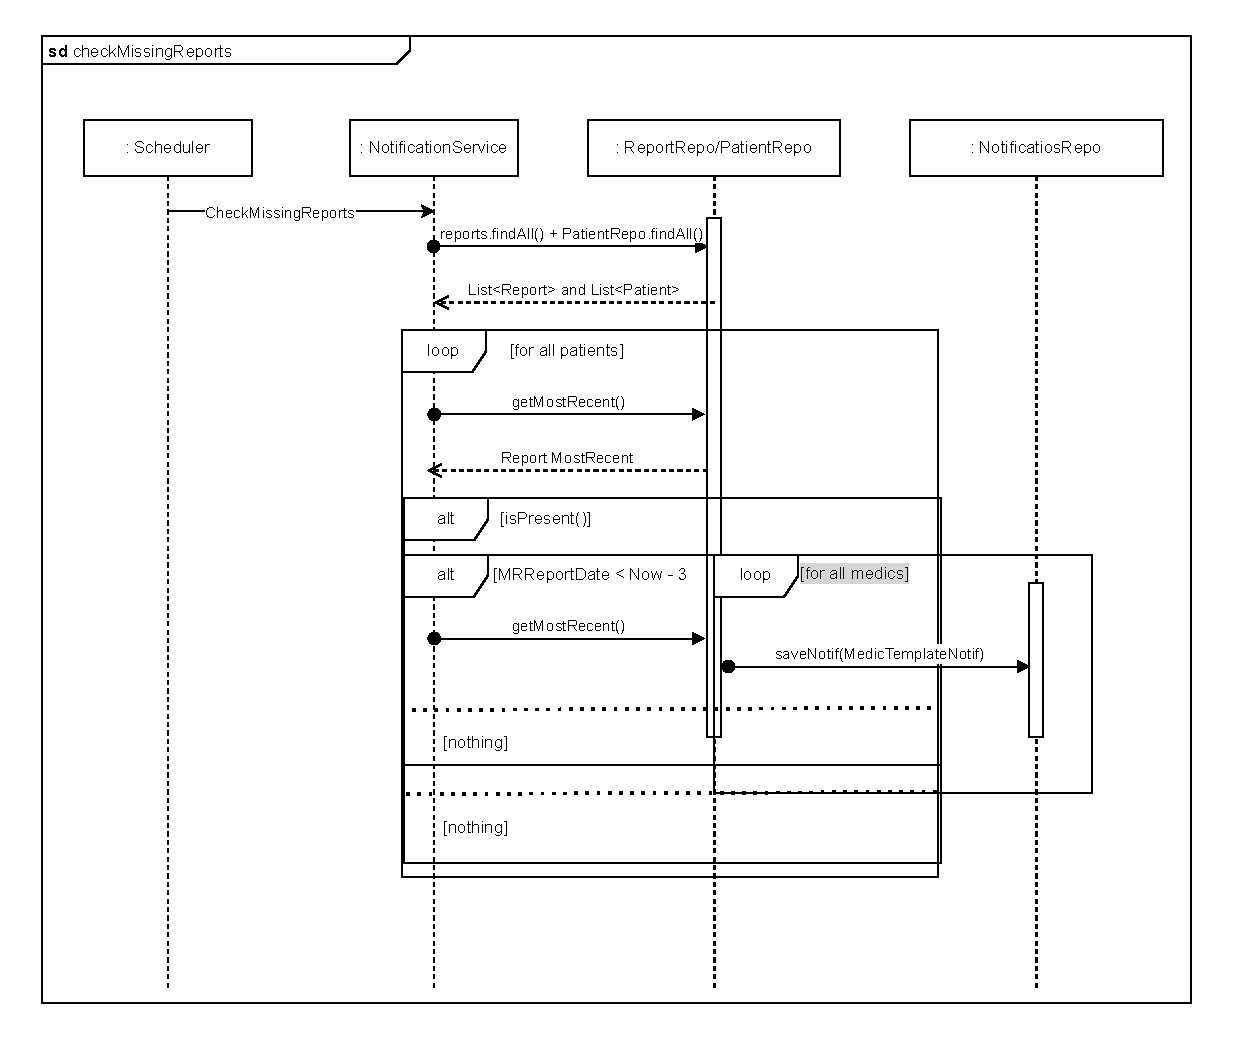
\includegraphics[width=1\textwidth]{checkMissingReports.pdf}
  \end{center}
  \caption{Sequence Diagram del controllo delle rilevazioni mancanti}  
\end{figure}
\noindent

\pagebreak

\section{Test e validazione}

Per testare il software sono stati utilizzati diversi tipi di test, tra cui:
\begin{itemize}
  \item Revisione del codice: il codice è stato revisionato da entrambi i membri del team per garantire che fosse scritto 
  in modo che rispettasse le specifiche del progetto e che fosse facilmente comprensibile.
  \item Verifica della consistenza: sono stati effettuati test per verificare che il software fosse coerente con le specifiche del progetto e che
  funzionasse come previsto, tramite i Bean @WebMvcTest di Spring Boot che permettono di testare i controller e le loro interazioni con il Model.
  Questo tipo di test è automatizzato grazie all'API di JUnit. 
  \item È stato usato @DataJpaTest per testare le interazioni con il database e verificare che le operazioni CRUD funzionassero correttamente.
  \item È stato fatto gran uso di Postman per testare le API REST del software, verificando che le richieste HTTP restituissero i risultati attesi.
  \item Il software è stato testato dagli sviluppatori
  \item Il software è stato testato da un utente generico
\end{itemize}

\subsection{Revisione del codice}

La fase di revisione del codice è stata effettuata da entrambi i membri del team, che hanno esaminato il codice 
per garantire che fosse scritto in modo chiaro e comprensibile e che soprattutto rispettasse le specifiche 
del progetto. Si è più volte controllato che gli use case, activity diagram, design pattern e sequence diagram 
fossero rispettati e che il codice fosse ben strutturato e organizzato. È stato rivisto il codice anche per 
cercare di trovare eventuali bug o errori di logica, in modo da correggerli prima di procedere con i test veri e propri.
Abbiamo dato più attenzione specialmente agli use case del paziente e del medico (insieme a quello che
può fare solo l'amministratore), in quanto sono le funzionalità principali del software.

\subsection{Test con @WebMvcTest e @DataJpaTest}

Per testare il software sono stati utilizzati i Bean di Spring Boot @WebMvcTest e @DataJpaTest, che permettono di testare i controller 
e le interazioni con un database di test salvato in memoria. Quello che segue 
è un esempio di test per il repository del paziente, che verifica le operazioni CRUD (Create, Read, Update, Delete).
Le funzioni con il tag @Test sono i test veri e propri e ad ogni test è stato assegnato un ordine tramite l'annotazione @Order.
Effettuiamo l'azione e verifichiamo che il risultato sia quello atteso, utilizzando le asserzioni di JUnit.

\begin{minted}{java}  
@DataJpaTest
@TestMethodOrder(MethodOrderer.OrderAnnotation.class)
public class PatientRepositoryTest {
  @Autowired
  private PatientRepository patientRepository;

  @Test
  @Order(1)
  @Rollback(value = false)
  public void createPatientTest() {

    // Action
    Patient patient = new Patient(new User("testmail", "pass", Role.PATIENT,true),
            "TestFirstName", "TestLastName",
        LocalDate.of(2000, 1, 1), new Medic(new User("medicmail",
            "pass", Role.MEDIC, true), "TestMedic", "lastname"));
    patientRepository.save(patient);

    // Verify
    System.out.println(patient);
    assertThat(patient.getId()).isGreaterThan(0);
  }

  @Test
  @Order(2)
  public void getPatientByIdTest() {
    // Action
    Patient found = patientRepository.findById(1).get();

    // Verify
    System.out.println(found);
    assertThat(found.getId()).isEqualTo(1);
  }

  @Test
  @Order(3)
  public void getAllPatientsTest() {
    // Action
    List<Patient> patients = patientRepository.findAll();

    // Verify
    System.out.println(patients);
    assertThat(patients.size()).isGreaterThan(0);
  }

  @Test
  @Order(4)
  @Rollback(value = false)
  public void updatePatientTest() {
    // Action
    Patient patient = patientRepository.findById(1).get();
    patient.setFirstName("UpdatedFirstName");
    patient.setLastName("UpdatedLastName");
    Patient updated = patientRepository.save(patient);

    // Verify
    System.out.println(updated);
    assertThat(updated.getFirstName()).isEqualTo("UpdatedFirstName");
    assertThat(updated.getLastName()).isEqualTo("UpdatedLastName");
  }

  @Test
  @Order(5)
  @Rollback(value = false)
  public void deletePatientTest() {
    // Action
    Patient patient = patientRepository.findById(1).get();
    patientRepository.delete(patient);

    // Verify
    Patient deleted = patientRepository.findById(1).orElse(null);
    assertThat(deleted).isNull();
  }
}
\end{minted}
\noindent
Il prossimo codice invece è preso dal test di un controller, più precisamente il controller dei pazienti.
\begin{minted}{java}
@WebMvcTest(PatientController.class)
@TestMethodOrder(MethodOrderer.OrderAnnotation.class)
public class PatientControllerTest {

  @Autowired
  private MockMvc mockMvc;

  @MockitoBean
  private PatientService patientService;

  @Autowired
  private ObjectMapper objectMapper;

  private Patient patient;

  @BeforeEach
  public void setup() {
    patient = new Patient(new User("usermail", "pass1", Role.PATIENT,true),
            "Nome", "Cognome", LocalDate.of(2000, 1, 1),
        new Medic(new User("medicmail", "medicpass", Role.MEDIC, true),
                "FirstName", "LastName"));
    patient.setId(1); // Set a mock ID for testing
  }

  // Post Controller
  @Test
  @Order(1)
  public void createPatientTest() throws Exception {
    // precondition
    given(patientService.create(any(Patient.class))).willReturn(patient);

    // action
    ResultActions response = mockMvc.perform(post("/patients")
        .contentType(MediaType.APPLICATION_JSON)
        .content(objectMapper.writeValueAsString(patient)));

    // verify
    response.andDo(print()).andExpect(status().isCreated())
        .andExpect(jsonPath("$.firstName",
            is(patient.getFirstName())))
        .andExpect(jsonPath("$.lastName",
            is(patient.getLastName())))
        .andExpect(jsonPath("$.birthDate",
            is(patient.getBirthDate())))
        .andExpect(jsonPath("$.referralMedic.id", 
        is(patient.getReferralMedic().getId())));
  }

  // Get Controller
  @Test
  @Order(2)
  public void getAllPatientsTest() throws Exception {
    // precondition
    List<Patient> patientsList = new ArrayList<>();
    patientsList.add(patient);
    patientsList
        .add(
                new Patient(new User("testmail", "testpass", 
                        Role.PATIENT,true), "test",
                        "test", LocalDate.of(2000, 1, 1),
                new Medic(new User("testmedicmail", "testpass", Role.MEDIC, true),
                        "testMedic", "lastname")));
    given(patientService.getAll()).willReturn(patientsList);

    // action
    ResultActions response = mockMvc.perform(get("/patients"));

    // verify
    response.andExpect(status().isOk())
        .andDo(print())
        .andExpect(jsonPath("$.size()",
            is(patientsList.size())));
  }

  @Test
  @Order(3)
  public void getPatientByIdTest() throws Exception {
    // precondition
    given(patientService.getById(patient.getId())).willReturn(Optional.of(patient));

    // action
    ResultActions response = mockMvc.perform(get("/patients/{id}", patient.getId()));

    // verify
    response.andExpect(status().isOk())
        .andDo(print())
        .andExpect(jsonPath("$.firstName",
            is(patient.getFirstName())))
        .andExpect(jsonPath("$.lastName",
            is(patient.getLastName())))
        .andExpect(jsonPath("$.birthDate",
            is(patient.getBirthDate())))
        .andExpect(jsonPath("$.referralMedic.id", 
        is(patient.getReferralMedic().getId())));
  }

  // Put Controller
  @Test
  @Order(4)
  public void updatePatientTest() throws Exception {
    // precondition
    patient.setFirstName("UpdatedFirst");
    patient.setLastName("UpdatedLast");
    given(patientService.update(any(Integer.class), 
    any(Patient.class))).willReturn(patient);

    // action
    ResultActions response = mockMvc.perform(put("/patients/{id}", patient.getId())
        .contentType(MediaType.APPLICATION_JSON)
        .content(objectMapper.writeValueAsString(patient)));

    // verify
    response.andExpect(status().isOk())
        .andDo(print())
        .andExpect(jsonPath("$.firstName",
            is(patient.getFirstName())))
        .andExpect(jsonPath("$.lastName",
            is(patient.getLastName())))
        .andExpect(jsonPath("$.birthDate",
            is(patient.getBirthDate())))
        .andExpect(jsonPath("$.referralMedic.id", 
        is(patient.getReferralMedic().getId())));
  }

  // Delete Controller
  @Test
  @Order(5)
  public void deletePatientTest() throws Exception {
    // precondition
    given(patientService.delete(patient.getId())).willReturn(patient);

    // action
    ResultActions response = mockMvc.perform(delete("/patients/{id}", patient.getId()));

    // verify
    response.andExpect(status().isOk())
        .andDo(print())
        .andExpect(jsonPath("$.firstName",
            is(patient.getFirstName())))
        .andExpect(jsonPath("$.lastName",
            is(patient.getLastName())))
        .andExpect(jsonPath("$.birthDate",
            is(patient.getBirthDate())))
        .andExpect(jsonPath("$.referralMedic.id", 
        is(patient.getReferralMedic().getId())));
  }

}
\end{minted}

\subsection{Postman}

Per \textbf{testare le API REST} del software, è stato utilizzato \textit{Postman}, un tool che permette di inviare richieste HTTP 
e di visualizzare le risposte. Ne è stato fatto un uso intensivo per testare le API del software,
poiché per testare le API REST è necessario inviare richieste HTTP e verificare le risposte.
Il nostro environment di Postman permette di simulare l'autenticazione degli utenti e di verificarne 
le funzionalità. Quando un utente si autentica, viene restituito un token JWT che viene utilizzato per
autenticare le richieste successive. Il token viene inserito nella cartella principale
dell'environment di Postman e viene utilizzato per autenticare le richieste da parte di tutti i controller.


\vspace{1em}
\noindent
Ovviamente per testare la correttezza generale del software in maniera veloce seguendo come sempre
uno stile \textit{Agile}, abbiamo creato un file java (\textit{LoadDatabase.java}) che carica in automatico i dati 
di test nel database,
in modo da poter testare le funzionalità del software senza dover inserire manualmente i dati.
Questa funzione di inizializzazione è stata rimossa quando il processo di sviluppo è stato ultimato per non
eliminare i dati dal database ogni volta che viene avviato il software.
Per ogni controller, sono stati creati dei test che verificano le funzionalità principali di essi, come 
la creazione, la lettura, l'aggiornamento e la cancellazione dei dati.
Postman ha aiutato incredibilmente anche a \textbf{testare che gli endpoints fossero protetti} correttamente e 
che le autorizzazioni funzionassero come previsto.

\begin{figure}[H]
  \begin{center}
    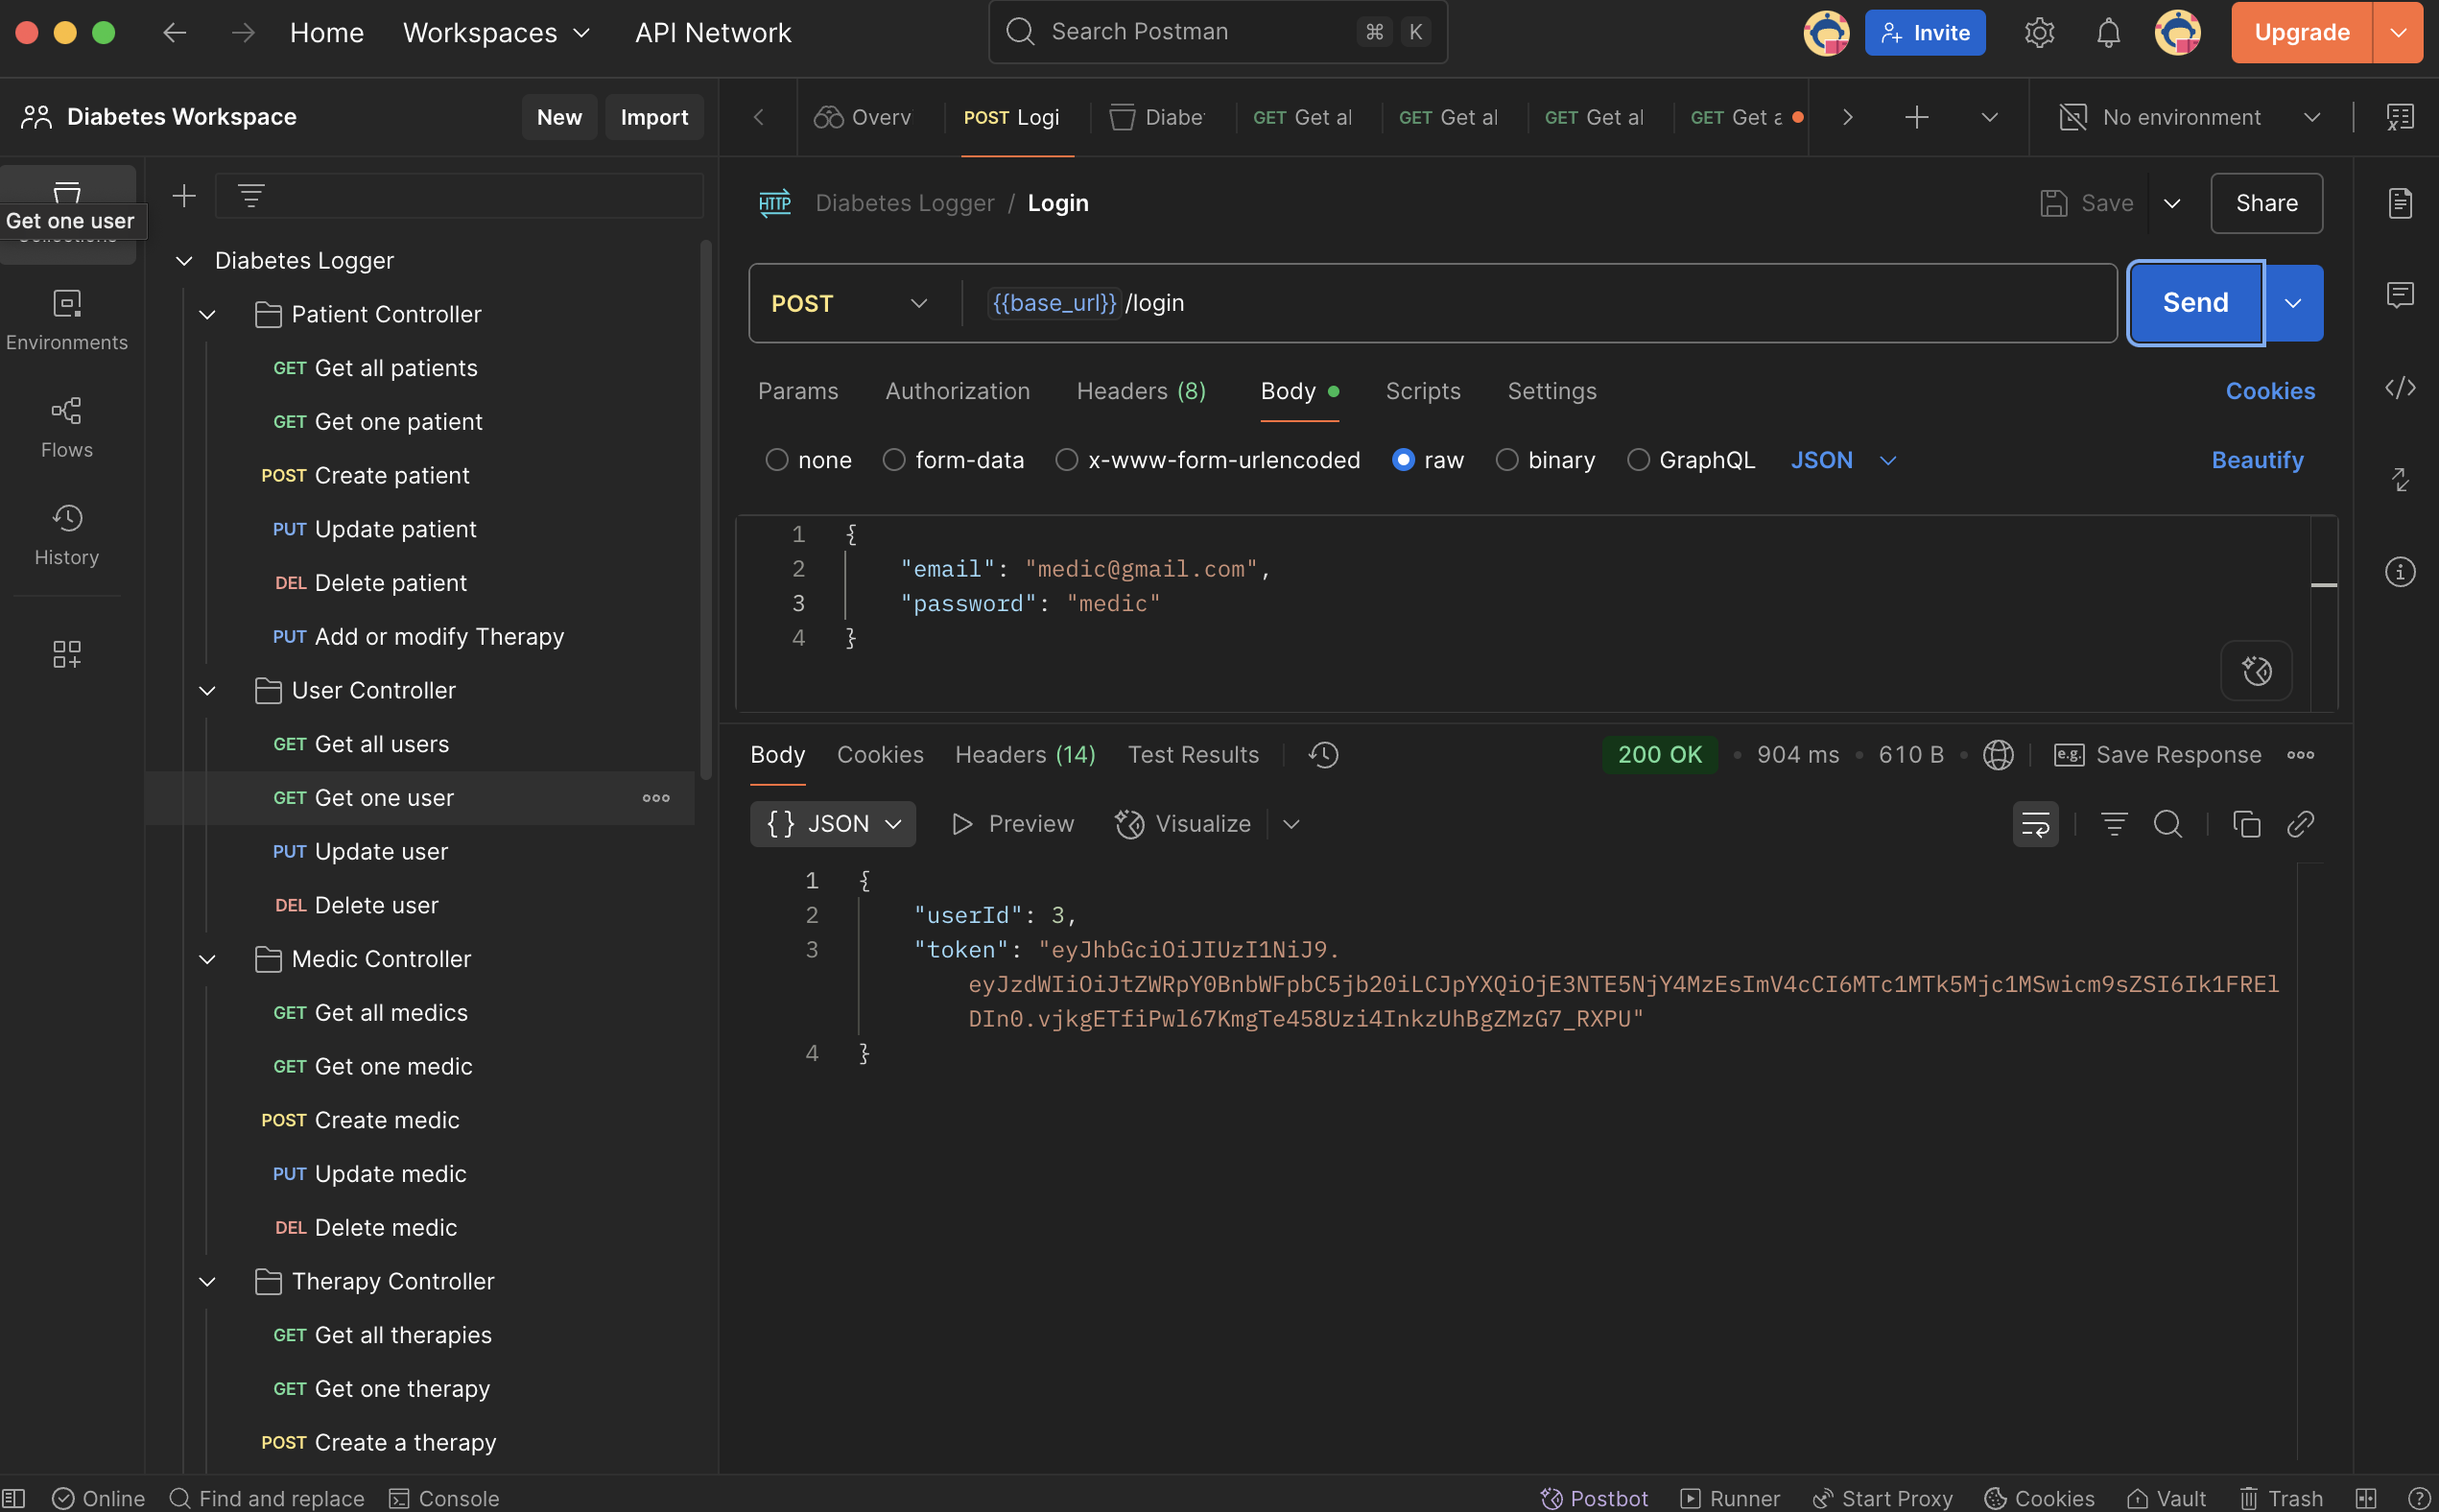
\includegraphics[width=1\textwidth]{postman.png}
  \end{center}
  \caption{Postman environment del progetto} 
  \label{fig:postman}
\end{figure}
\noindent


\subsection{Test manuali degli sviluppatori}

In questa fase ci siamo preoccupati di testare il software manualmente,
verificando che tutte le funzionalità implementate funzionassero come previsto e che non ci fossero bug o errori di logica.
Alcuni dei test effettuati sono stati:
\begin{itemize}
  \item Verifica che il login funzionasse correttamente per tutti gli utenti;
  \item Verifica che la registrazione funzionasse correttamente per tutti i ruoli;
  \item Verifica che l'utente potesse modificare i propri dati;
  \item I campi obbligatori devono essere riempiti correttamente
  altrimenti il Controller avvisa di riempirli;
  \item Alcuni campi non possono essere modificati da un certo tipo di utente 
  questo tipo di sicurezza è stata implementata tramite il pattern Security di Spring Boot
  e quindi è stato semplice accertarsi che funzionasse;
  \item Inserimento di un report con dati validi e verifica che venisse creato correttamente;
  \item Verifica che le notifiche vengano create correttamente quando un report 
  "preoccupante" viene inserito;
  \item Verifica che le notifiche vengano cancellate 
  correttamente quando un utente le cancella;
  \item Verificato che il sistema di avvisi tramite notifiche;
  \item Verifica dei vari inserimenti con input errati oppure vuoti;
  \item Verifica di un assegnazione di una terapia ad un paziente;
  \item Inserimento di terapie, pazienti o medici duplicati
  \item Verifica che l'amministratore potesse gestire gli utenti e le richieste di registrazione;
  \item Verifica che l'amministratore potesse visualizzare la traccia dei medici e i medici l'ultima 
  operazione effettuata su un paziente;
  \item Verificato che il paziente possa vedere solo i suoi report ma non quelli degli altri pazienti;
\end{itemize}

\subsection{Test utente generico}

Per testare il software da un utente generico, abbiamo chiesto ad un individuo esterno di provare 
il software e di darci un feedback sulle funzionalità implementate.
L'utente ha richiesto la registrazione di un nuovo account e ha provato a utilizzare il software come un paziente,
provando ad inserire report e visualizzare le notifiche.
Lo scopo di questo test era quello di verificare che il software fosse facile da usare e che 
le funzionalità implementate fossero intuitive.
Il feedback ricevuto è stato positivo e allo stesso tempo ci ha dato spunti
per migliorare ulteriormente l'usabilità del software. 


\end{document}
